%% This file was auto-generated by IPython.
%% Conversion from the original notebook file:
%% REDD_House2_Analysis.ipynb
%%
\documentclass[11pt,english]{article}

%% This is the automatic preamble used by IPython.  Note that it does *not*
%% include a documentclass declaration, that is added at runtime to the overall
%% document.

\usepackage{amsmath}
\usepackage{amssymb}
\usepackage{graphicx}
\usepackage{ucs}
\usepackage[utf8x]{inputenc}

% needed for markdown enumerations to work
\usepackage{enumerate}

% Slightly bigger margins than the latex defaults
\usepackage{geometry}
\geometry{verbose,tmargin=3cm,bmargin=3cm,lmargin=2.5cm,rmargin=2.5cm}

% Define a few colors for use in code, links and cell shading
\usepackage{color}
\definecolor{orange}{cmyk}{0,0.4,0.8,0.2}
\definecolor{darkorange}{rgb}{.71,0.21,0.01}
\definecolor{darkgreen}{rgb}{.12,.54,.11}
\definecolor{myteal}{rgb}{.26, .44, .56}
\definecolor{gray}{gray}{0.45}
\definecolor{lightgray}{gray}{.95}
\definecolor{mediumgray}{gray}{.8}
\definecolor{inputbackground}{rgb}{.95, .95, .85}
\definecolor{outputbackground}{rgb}{.95, .95, .95}
\definecolor{traceback}{rgb}{1, .95, .95}

% Framed environments for code cells (inputs, outputs, errors, ...).  The
% various uses of \unskip (or not) at the end were fine-tuned by hand, so don't
% randomly change them unless you're sure of the effect it will have.
\usepackage{framed}

% remove extraneous vertical space in boxes
\setlength\fboxsep{0pt}

% codecell is the whole input+output set of blocks that a Code cell can
% generate.

% TODO: unfortunately, it seems that using a framed codecell environment breaks
% the ability of the frames inside of it to be broken across pages.  This
% causes at least the problem of having lots of empty space at the bottom of
% pages as new frames are moved to the next page, and if a single frame is too
% long to fit on a page, will completely stop latex from compiling the
% document.  So unless we figure out a solution to this, we'll have to instead
% leave the codecell env. as empty.  I'm keeping the original codecell
% definition here (a thin vertical bar) for reference, in case we find a
% solution to the page break issue.

%% \newenvironment{codecell}{%
%%     \def\FrameCommand{\color{mediumgray} \vrule width 1pt \hspace{5pt}}%
%%    \MakeFramed{\vspace{-0.5em}}}
%%  {\unskip\endMakeFramed}

% For now, make this a no-op...
\newenvironment{codecell}{}

 \newenvironment{codeinput}{%
   \def\FrameCommand{\colorbox{inputbackground}}%
   \MakeFramed{\advance\hsize-\width \FrameRestore}}
 {\unskip\endMakeFramed}

\newenvironment{codeoutput}{%
   \def\FrameCommand{\colorbox{outputbackground}}%
   \vspace{-1.4em}
   \MakeFramed{\advance\hsize-\width \FrameRestore}}
 {\unskip\medskip\endMakeFramed}

\newenvironment{traceback}{%
   \def\FrameCommand{\colorbox{traceback}}%
   \MakeFramed{\advance\hsize-\width \FrameRestore}}
 {\endMakeFramed}

% Use and configure listings package for nicely formatted code
\usepackage{listingsutf8}
\lstset{
  language=python,
  inputencoding=utf8x,
  extendedchars=\true,
  aboveskip=\smallskipamount,
  belowskip=\smallskipamount,
  xleftmargin=2mm,
  breaklines=true,
  basicstyle=\small \ttfamily,
  showstringspaces=false,
  keywordstyle=\color{blue}\bfseries,
  commentstyle=\color{myteal},
  stringstyle=\color{darkgreen},
  identifierstyle=\color{darkorange},
  columns=fullflexible,  % tighter character kerning, like verb
}

% The hyperref package gives us a pdf with properly built
% internal navigation ('pdf bookmarks' for the table of contents,
% internal cross-reference links, web links for URLs, etc.)
\usepackage{hyperref}
\hypersetup{
  breaklinks=true,  % so long urls are correctly broken across lines
  colorlinks=true,
  urlcolor=blue,
  linkcolor=darkorange,
  citecolor=darkgreen,
  }

% hardcode size of all verbatim environments to be a bit smaller
\makeatletter 
\g@addto@macro\@verbatim\small\topsep=0.5em\partopsep=0pt
\makeatother 

% Prevent overflowing lines due to urls and other hard-to-break entities.
\sloppy

\begin{document}

\section{Non Intrusive Load Monitoring on REDD dataset}
\paragraph{Version 0.2}
Changelog

\begin{itemize}
\item
  Now uses Pandas for resampling, indexing, and most other Time Series
  operations.This fixes a bug earlier, where we downsampled based on the
  number of samples and not on the basis of time
\item
  Added breakdown by time analsyis showing daily variation and 6 hourly
  variation, also weekday vs weekend
\item
  Added pie-chart breakdown by appliance analysis
\item
  Added dataframe capability, using Pandas which also gives high level
  overview of the data
\item
  Added a much quicker implementation of KMeans and also compared with
  Mini Batch KMeans
\end{itemize}

\subsection{About the dataset}
The datset contains high frequency, low frequency and raw data of 6
households in the USA. We choose House 2 for our analysis as it contains
the least number of appliances. Further we choose to do the analysis of
\textbf{low frequency} data. This house contains the following
appliances/circuits:

\begin{itemize}
\item
  Kitchen
\item
  Kitchen 2
\item
  Stove
\item
  Refrigerator
\item
  Dishwasher
\item
  Disposal
\item
  Washer Dryer
\item
  Microwave
\item
  Lighting
\end{itemize}

These circuits are samppled once every 3-4 seconds. Also the house
contains 2 mains which are sampled at 1 Hz.

\subsection{Basic imports}
In this section we setup the basic imports which shall be required for
performing the analysis.

\begin{codecell}
\begin{codeinput}
\begin{lstlisting}
import numpy as np
import matplotlib.pyplot as plt
import math
from scipy.cluster.vq import kmeans,vq
import itertools
import matplotlib
#Setting size of figures as 20*10
plt.figsize(20,10)
#Setting font size to be 16
matplotlib.rcParams.update({'font.size': 16})
import pandas as pd
from pandas import Series,DataFrame
plt.figsize(20,10)
import json
s = json.load( open("/home/nipun/bmh_matplotlibrc.json") )
matplotlib.rcParams.update(s)
matplotlib.rcParams.update({'font.size': 16})
import time
\end{lstlisting}
\end{codeinput}
\end{codecell}
\subsection{Loading and Plotting of Mains  Data}
\begin{codecell}
\begin{codeinput}
\begin{lstlisting}
start_time=time.time()
mains_1_data=np.loadtxt('/home/nipun/study/datasets/MIT/low_freq/house_2/channel_1.dat')
mains_2_data=np.loadtxt('/home/nipun/study/datasets/MIT/low_freq/house_2/channel_2.dat')
end_time=time.time()
print "Time taken to load Mains data= "+str(end_time-start_time)+" seconds"
\end{lstlisting}
\end{codeinput}
\begin{codeoutput}
\begin{verbatim}
Time taken to load Mains data= 23.7791380882 seconds
\end{verbatim}
\end{codeoutput}
\end{codecell}
We can observe that data is missing towards the end. As a part of the
data cleansing process we should eliminate the last indices. Next we
find the last valid index for which contiguos data is present.This
corresponds to epoch timestamp of 1304282291.

\begin{codecell}
\begin{codeinput}
\begin{lstlisting}
upper=np.where(mains_1_data[:,0]==1304282291.0)[0]
lower=np.where(mains_1_data[:,0]>1303084800.0)[0][0]
mains_1_power=mains_1_data[:,1][lower:upper]
mains_2_power=mains_2_data[:,1][lower:upper]
timestamp=mains_1_data[:,0][lower:upper]
timestamp_mains_date=timestamp.astype('datetime64[s]')
\end{lstlisting}
\end{codeinput}
\end{codecell}
Overall statistics about the dataset.

\begin{codecell}
\begin{codeinput}
\begin{lstlisting}
df_mains=DataFrame({'Mains_1_Power':mains_1_power,'Mains_2_Power':mains_2_power},index=timestamp_mains_date)
df_mains.describe()
\end{lstlisting}
\end{codeinput}
\begin{codeoutput}
\begin{verbatim}
        Mains_1_Power   Mains_2_Power
count  1162980.000000  1162980.000000
mean        43.401942      187.478237
std        148.175308      213.889966
min         12.270000       21.190000
25%         14.830000       22.470000
50%         15.110000      218.380000
75%         33.510000      259.160000
max       1887.420000     3149.020000
\end{verbatim}
\end{codeoutput}
\end{codecell}
Plotting overall power consumption for the two main circuits.

\begin{codecell}
\begin{codeinput}
\begin{lstlisting}
start_time=time.time()
df_mains.plot(subplots=True,title='Power consumption');
end_time=time.time()
print "Time taken to plot Mains data= "+str(end_time-start_time)+" seconds"
\end{lstlisting}
\end{codeinput}
\begin{codeoutput}
\begin{verbatim}
Time taken to plot Mains data= 12.8343689442 seconds
\end{verbatim}
\begin{center}
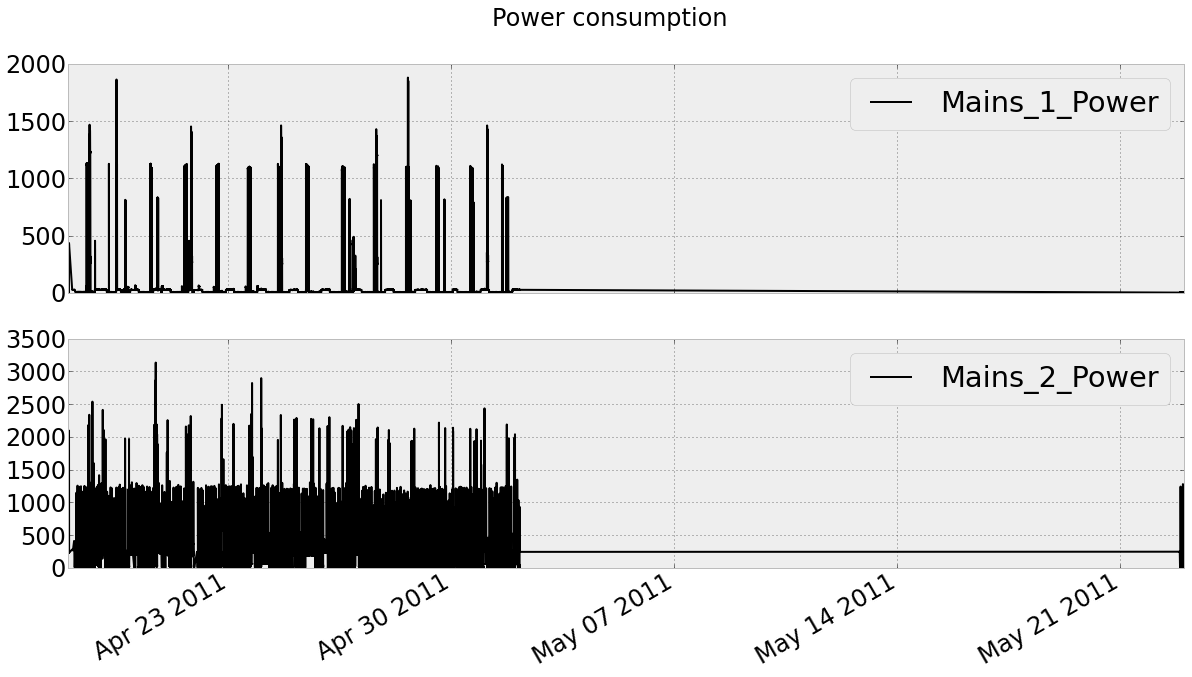
\includegraphics[width=0.7\textwidth]{REDD_House2_Analysis_files/REDD_House2_Analysis_fig_00.png}
\par
\end{center}
\end{codeoutput}
\end{codecell}
\subsection{Downsampling Mains Data}
\begin{codecell}
\begin{codeinput}
\begin{lstlisting}
start_time=time.time()
df_1_day=df_mains.resample('1d',how='sum');
df_1_day_energy=DataFrame(index=df_1_day.index);
df_1_day_energy['Mains_1_Energy']=Series(df_1_day.Mains_1_Power/(1000*3600),index=df_1_day.index)
df_1_day_energy['Mains_2_Energy']=Series(df_1_day.Mains_2_Power/(1000*3600),index=df_1_day.index)
end_time=time.time()
print "Time taken to resample Mains data= "+str(end_time-start_time)+" seconds"
\end{lstlisting}
\end{codeinput}
\begin{codeoutput}
\begin{verbatim}
Time taken to resample Mains data= 0.0693271160126 seconds
\end{verbatim}
\end{codeoutput}
\end{codecell}
Energy consumption (KWh) statistics about data.

\begin{codecell}
\begin{codeinput}
\begin{lstlisting}
df_1_day_energy.describe()
\end{lstlisting}
\end{codeinput}
\begin{codeoutput}
\begin{verbatim}
       Mains_1_Energy  Mains_2_Energy
count       14.000000       14.000000
mean         1.001500        4.326060
std          0.284175        0.739165
min          0.739473        3.243120
25%          0.766775        3.733631
50%          0.870461        4.329253
75%          1.264915        4.907687
max          1.516066        5.567054
\end{verbatim}
\end{codeoutput}
\end{codecell}
Plotting daily energy consumption.

\begin{codecell}
\begin{codeinput}
\begin{lstlisting}
def correct_labels(ax):
    labels = [item.get_text() for item in ax.get_xticklabels()]
    days=[label.split(" ")[0] for label in labels]
    months=["Jan","Feb","Mar","Apr","May","Jun","Jul","Aug","Sep","Oct","Nov","Dec"]
    final_labels=[]
    for i in range(len(days)):
        a=days[i].split("-")
        final_labels.append(a[2]+"\n"+months[int(a[1])-1])
    ax.set_xticklabels(final_labels)
\end{lstlisting}
\end{codeinput}
\end{codecell}
Function to find which of the days are weekdays and their indices

\begin{codecell}
\begin{codeinput}
\begin{lstlisting}
def find_weekend_indices(datetime_array):
    indices=[]
    for i in range(len(datetime_array)):
        if datetime_array[i].weekday()>=5:
            indices.append(i)
    return indices
def highlight_weekend(weekend_indices,ax,ymax):
    i=0
    while i<len(weekend_indices):
        ax.fill_between([weekend_indices[i],weekend_indices[i]+2],ymax,facecolor='green',alpha=.2)    
        i+=2
        
\end{lstlisting}
\end{codeinput}
\end{codecell}
\begin{codecell}
\begin{codeinput}
\begin{lstlisting}
date_range=[datetime.datetime(2011,4,18)+datetime.timedelta(days=i) for i in range(14)]
weekend_indices=find_weekend_indices(date_range)
\end{lstlisting}
\end{codeinput}
\end{codecell}
\begin{codecell}
\begin{codeinput}
\begin{lstlisting}
ax=df_1_day_energy.plot(kind='bar',rot=0);
ax.set_title('Energy Consumption Per Day Home II');
ax.set_ylabel('Energy (KWh)');
correct_labels(ax);
highlight_weekend(weekend_indices,ax,6);
\end{lstlisting}
\end{codeinput}
\begin{codeoutput}
\begin{center}
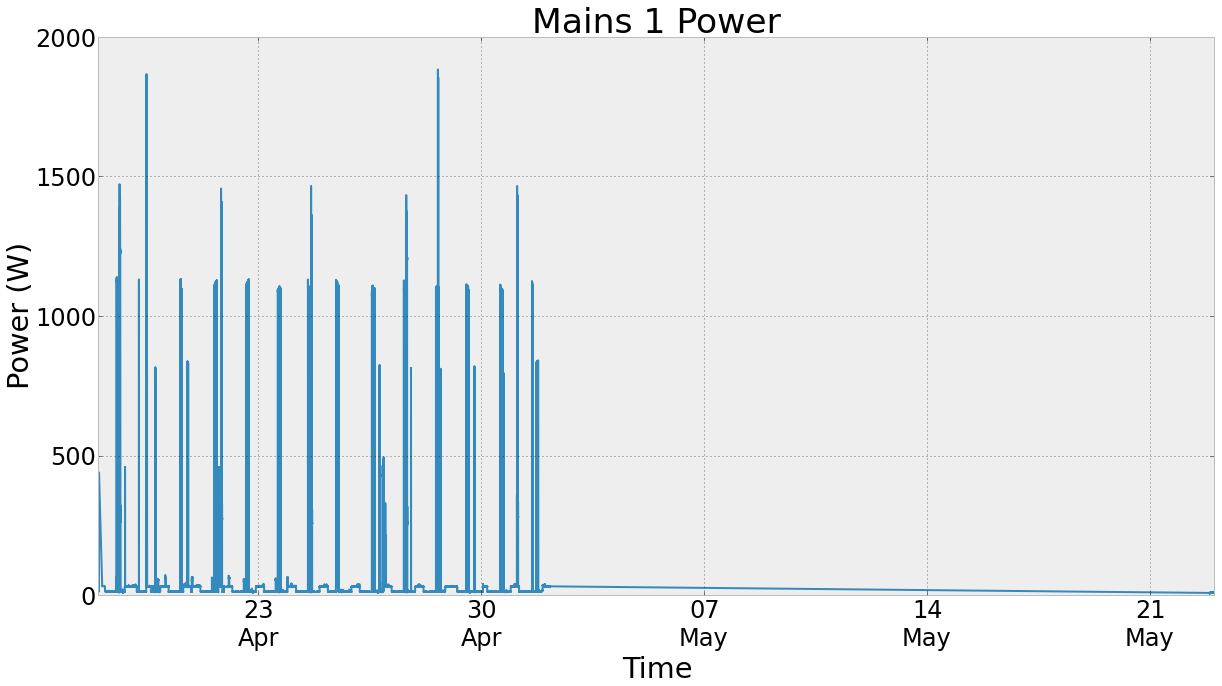
\includegraphics[width=0.7\textwidth]{REDD_House2_Analysis_files/REDD_House2_Analysis_fig_01.png}
\par
\end{center}
\end{codeoutput}
\end{codecell}
\begin{codecell}
\begin{codeinput}
\begin{lstlisting}
ax=df_1_day_energy.plot(kind='bar',stacked=True,rot=0);
ax.set_title('Energy Consumption Per Day Home II');
ax.set_ylabel('Energy (KWh)');
correct_labels(ax);
highlight_weekend(weekend_indices,ax,7);
\end{lstlisting}
\end{codeinput}
\begin{codeoutput}
\begin{center}
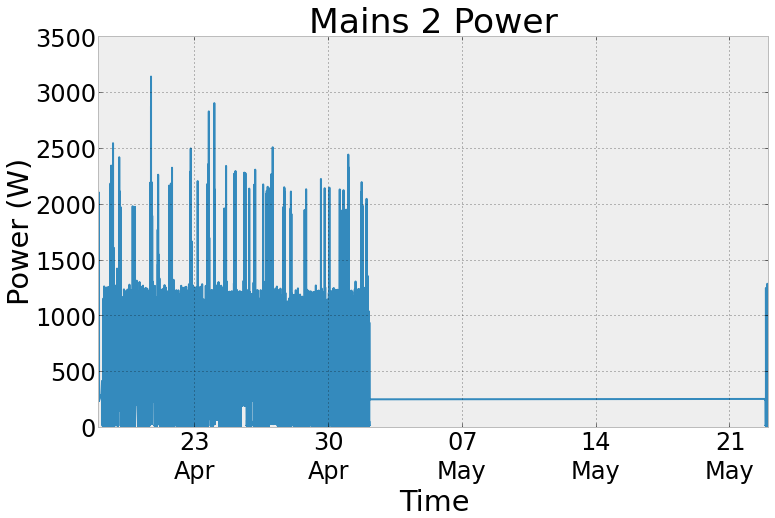
\includegraphics[width=0.7\textwidth]{REDD_House2_Analysis_files/REDD_House2_Analysis_fig_02.png}
\par
\end{center}
\end{codeoutput}
\end{codecell}
Now we try to break down the energy consumption into 6 hours slot and
see if we can see some patterns amongst the same.

\begin{codecell}
\begin{codeinput}
\begin{lstlisting}
df_6_hours=df_mains.resample('6h',how='sum');
df_6_hours_energy=DataFrame(index=df_6_hours.index);
df_6_hours_energy['Mains_1_Energy']=Series(df_6_hours.Mains_1_Power/(1000*3600),index=df_6_hours.index)
df_6_hours_energy['Mains_2_Energy']=Series(df_6_hours.Mains_2_Power/(1000*3600),index=df_6_hours.index)
\end{lstlisting}
\end{codeinput}
\end{codecell}
Statistics about Energy data downsampled to 6 hours.

\begin{codecell}
\begin{codeinput}
\begin{lstlisting}
df_6_hours_energy.describe()
\end{lstlisting}
\end{codeinput}
\begin{codeoutput}
\begin{verbatim}
       Mains_1_Energy  Mains_2_Energy
count       56.000000       56.000000
mean         0.250375        1.081515
std          0.228078        0.439292
min          0.028911        0.235619
25%          0.107926        0.762373
50%          0.162402        0.964794
75%          0.305203        1.386838
max          0.983501        2.117311
\end{verbatim}
\end{codeoutput}
\end{codecell}
\begin{codecell}
\begin{codeinput}
\begin{lstlisting}
days_mains_1=[]
dawn_mains_1=[]
morning_mains_1=[]
dusk_mains_1=[]
night_mains_1=[]
dawn_mains_2=[]
morning_mains_2=[]
dusk_mains_2=[]
night_mains_2=[]
for i in range(len(df_6_hours_energy.Mains_1_Energy)/4):
    days_mains_1.append(df_6_hours_energy.index[4*i])
    dawn_mains_1.append(df_6_hours_energy.Mains_1_Energy[4*i])
    morning_mains_1.append(df_6_hours_energy.Mains_1_Energy[4*i+1])
    dusk_mains_1.append(df_6_hours_energy.Mains_1_Energy[4*i+2])
    night_mains_1.append(df_6_hours_energy.Mains_1_Energy[4*i+3])   
    dawn_mains_2.append(df_6_hours_energy.Mains_2_Energy[4*i])
    morning_mains_2.append(df_6_hours_energy.Mains_2_Energy[4*i+1])
    dusk_mains_2.append(df_6_hours_energy.Mains_2_Energy[4*i+2])
    night_mains_2.append(df_6_hours_energy.Mains_2_Energy[4*i+3])
\end{lstlisting}
\end{codeinput}
\end{codecell}
Plotting 6 hourly breakdown of energy consumption from Mains 1

\begin{codecell}
\begin{codeinput}
\begin{lstlisting}
df4=DataFrame({'1':dawn_mains_1,'2':morning_mains_1,'3':dusk_mains_1,'4':night_mains_1},index=days_mains_1)
ax=df4.plot(kind='bar',stacked=False,legend=False,rot=0);
patches, labels = ax.get_legend_handles_labels();
ax.legend(patches, labels, loc='upper right');
ax.set_title('6 hourly Breakdown of energy consumption Mains 1');
ax.set_ylabel('Energy (KWh)');
correct_labels(ax);
highlight_weekend(weekend_indices,ax,1);
\end{lstlisting}
\end{codeinput}
\begin{codeoutput}
\begin{center}
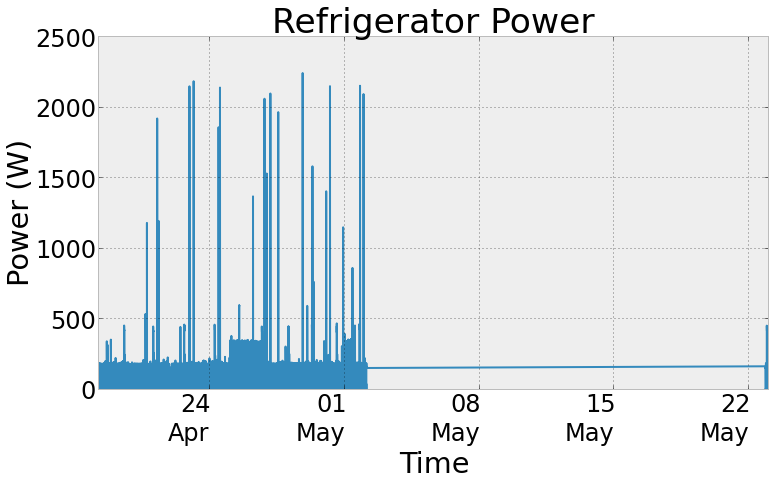
\includegraphics[width=0.7\textwidth]{REDD_House2_Analysis_files/REDD_House2_Analysis_fig_03.png}
\par
\end{center}
\end{codeoutput}
\end{codecell}
\begin{codecell}
\begin{codeinput}
\begin{lstlisting}
#ax.fill_between(pd.date_range("2011-4-18","2011-4-24"),0,20)
df4=DataFrame({'1':dawn_mains_1,'2':morning_mains_1,'3':dusk_mains_1,'4':night_mains_1},index=days_mains_1)
ax=df4.plot(kind='bar',stacked=True,legend=False,rot=0);
#ax.fill_between(pd.date_range("2011-4-18","2011-4-24"),0,20);
patches, labels = ax.get_legend_handles_labels();
ax.legend(patches, labels, loc='upper right');
ax.set_title('6 hourly breakdown of energy consumption Mains 1');
ax.set_ylabel('Energy (KWh)');
correct_labels(ax);
highlight_weekend(weekend_indices,ax,1.6);
\end{lstlisting}
\end{codeinput}
\begin{codeoutput}
\begin{center}
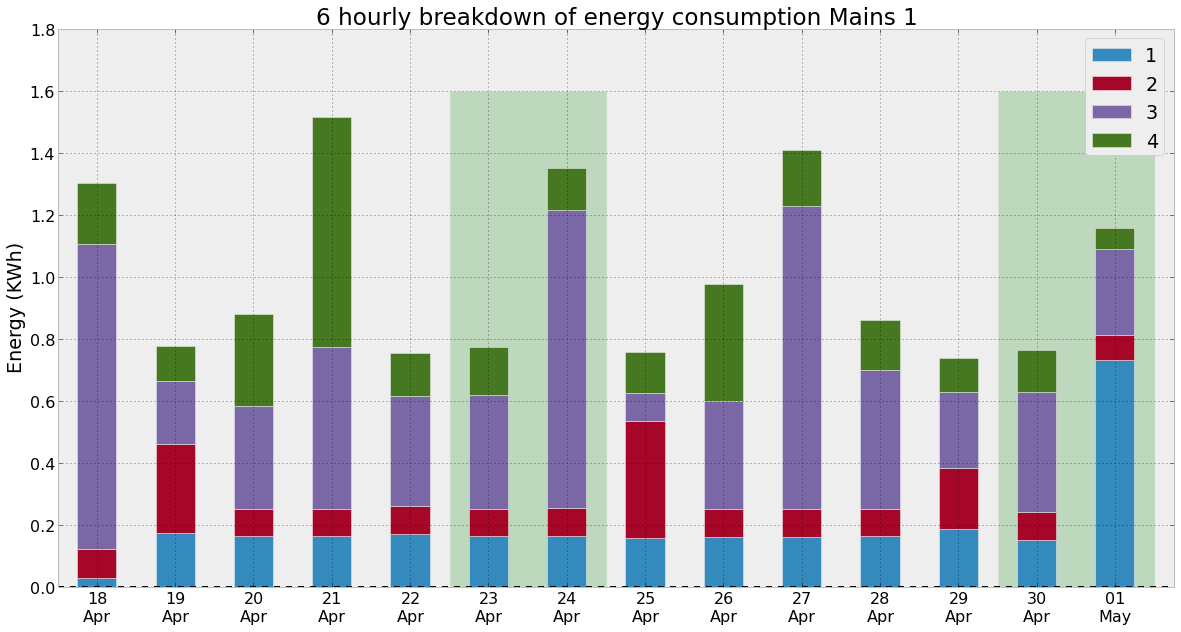
\includegraphics[width=0.7\textwidth]{REDD_House2_Analysis_files/REDD_House2_Analysis_fig_04.png}
\par
\end{center}
\end{codeoutput}
\end{codecell}
\begin{codecell}
\begin{codeinput}
\begin{lstlisting}
df5=DataFrame({'1':dawn_mains_2,'2':morning_mains_2,'3':dusk_mains_2,'4':night_mains_2},index=days_mains_1)
ax=df5.plot(kind='bar',stacked=False,legend=False,rot=0);
patches, labels = ax.get_legend_handles_labels();
ax.legend(patches, labels, loc='upper right');
ax.set_title('6 hourly Breakdown of energy consumption Mains 2');
ax.set_ylabel('Energy (KWh)');
correct_labels(ax);
highlight_weekend(weekend_indices,ax,2.5);
\end{lstlisting}
\end{codeinput}
\begin{codeoutput}
\begin{center}
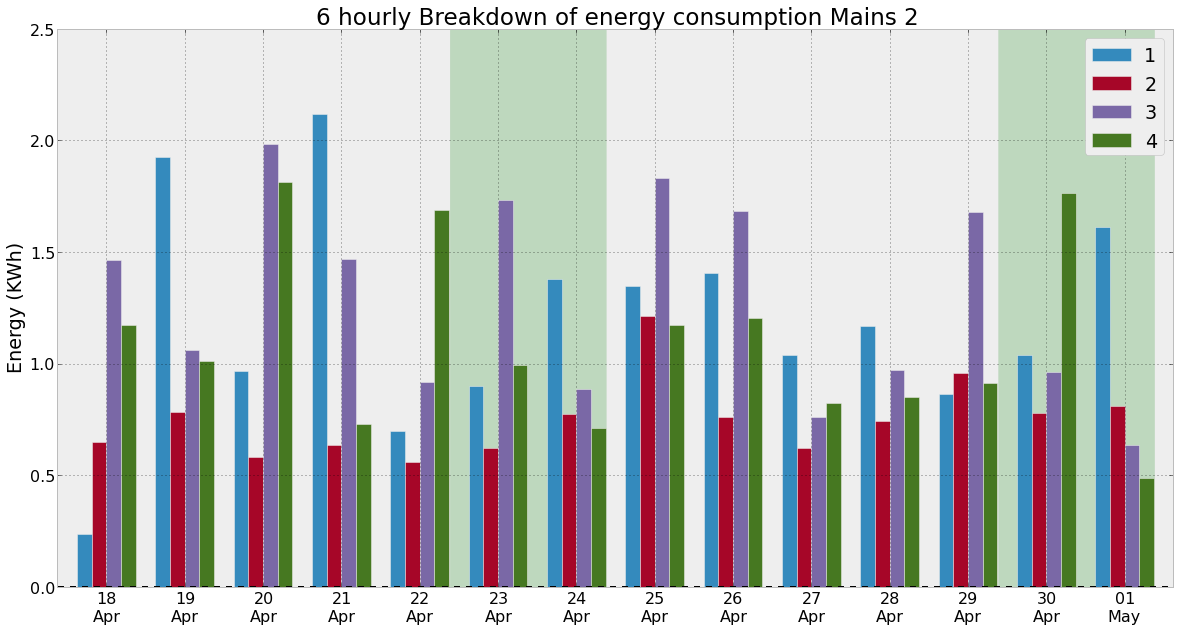
\includegraphics[width=0.7\textwidth]{REDD_House2_Analysis_files/REDD_House2_Analysis_fig_05.png}
\par
\end{center}
\end{codeoutput}
\end{codecell}
\begin{codecell}
\begin{codeinput}
\begin{lstlisting}
ax=df5.plot(kind='bar',stacked=True,legend=False,rot=0);
patches, labels = ax.get_legend_handles_labels();
ax.legend(patches, labels, loc='upper right');
ax.set_title('6 hourly Breakdown of energy consumption Mains 2');
ax.set_ylabel('Energy (KWh)');
correct_labels(ax);
highlight_weekend(weekend_indices,ax,6);
\end{lstlisting}
\end{codeinput}
\begin{codeoutput}
\begin{center}
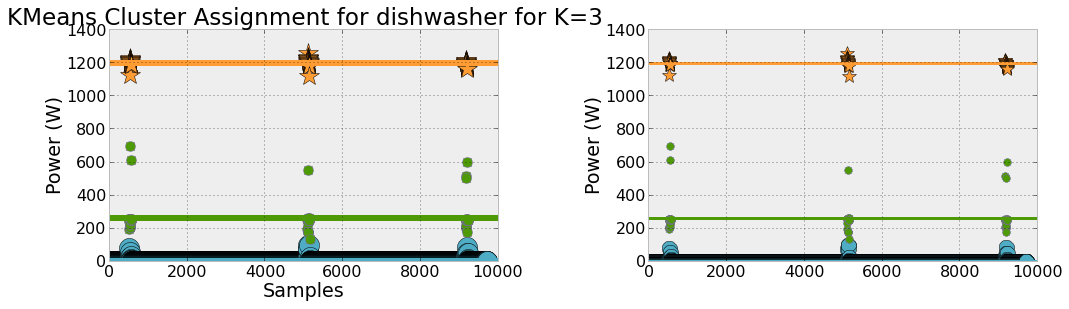
\includegraphics[width=0.7\textwidth]{REDD_House2_Analysis_files/REDD_House2_Analysis_fig_06.png}
\par
\end{center}
\end{codeoutput}
\end{codecell}
\begin{codecell}
\begin{codeinput}
\begin{lstlisting}
start_time=time.time()
kitchen_data=np.loadtxt('house_2/channel_3.dat')
light_data=np.loadtxt('house_2/channel_4.dat')
stove_data=np.loadtxt('house_2/channel_5.dat')
microwave_data=np.loadtxt('house_2/channel_6.dat')
washer_dry_data=np.loadtxt('house_2/channel_7.dat')
kitchen_2_data=np.loadtxt('house_2/channel_8.dat')
refrigerator_data=np.loadtxt('house_2/channel_9.dat')
dishwasher_data=np.loadtxt('house_2/channel_10.dat')
disposal_data=np.loadtxt('house_2/channel_11.dat')
upper=np.where(kitchen_data[:,0]==1304282291.0)[0]
lower=np.where(mains_1_data[:,0]>1303084800.0)[0][0]
kitchen_power=kitchen_data[:,1][lower:upper]
light_power=light_data[:,1][lower:upper]
stove_power=stove_data[:,1][lower:upper]
microwave_power=microwave_data[:,1][lower:upper]
washer_dryer_power=washer_dry_data[:,1][lower:upper]
kitchen_2_power=kitchen_2_data[:,1][lower:upper]
refrigerator_power=refrigerator_data[:,1][lower:upper]
dishwasher_power=dishwasher_data[:,1][lower:upper]
disposal_power=disposal_data[:,1][lower:upper]
timestamp=kitchen_data[:,0][lower:upper]
timestamp_appliance_date=timestamp.astype('datetime64[s]')
end_time=time.time()
print "Time taken to load appliance data= "+str(end_time-start_time)+" seconds"
\end{lstlisting}
\end{codeinput}
\begin{codeoutput}
\begin{verbatim}
Time taken to load appliance data= 28.4558880329 seconds
\end{verbatim}
\end{codeoutput}
\end{codecell}
\begin{codecell}
\begin{codeinput}
\begin{lstlisting}
df_appliances=DataFrame({'kitchen':kitchen_power,'light':light_power,'stove':stove_power,'microwave':microwave_power,\
'washer_dryer':washer_dryer_power,'kitchen_2':kitchen_2_power,'refrigerator':refrigerator_power,'dishwasher':dishwasher_power,\
'disposal':disposal_power},index=timestamp_appliance_date)
pd.set_option('display.precision', 2)
print df_appliances.describe().to_string()
\end{lstlisting}
\end{codeinput}
\begin{codeoutput}
\begin{verbatim}
dishwasher  disposal   kitchen  kitchen_2     light  microwave  refrigerator     stove  washer_dryer
count    308612.0  308612.0  308612.0   308612.0  308612.0   308612.0      308612.0  308612.0      308612.0
mean          9.2       0.1       6.1       10.5      26.9       14.4          79.6       1.5           2.2
std          97.2       3.4      38.3       99.0      46.2      104.5          87.7      19.2           0.7
min           0.0       0.0       0.0        0.0       0.0        0.0           0.0       0.0           0.0
25%           0.0       0.0       0.0        1.0       8.0        4.0           6.0       0.0           2.0
50%           0.0       0.0       0.0        1.0       8.0        5.0           7.0       0.0           2.0
75%           0.0       0.0      13.0        1.0       9.0        5.0         161.0       1.0           2.0
max        1457.0     609.0     805.0     1119.0     289.0     1986.0        2246.0     457.0          55.0
\end{verbatim}
\end{codeoutput}
\end{codecell}
Now we plot all the channels and describe their statistics

\begin{codecell}
\begin{codeinput}
\begin{lstlisting}
import matplotlib.pyplot as plt
start_time=time.time()
ax=df_appliances.plot(subplots=True,title="Appliance Power consumption",fontsize=10,figsize=(20,40))
plt.tight_layout()
end_time=time.time()
print "Time taken to plot appliance data= "+str(end_time-start_time)+" seconds"
\end{lstlisting}
\end{codeinput}
\begin{codeoutput}
\begin{verbatim}
Time taken to plot appliance data= 16.4023768902 seconds
\end{verbatim}
\begin{center}
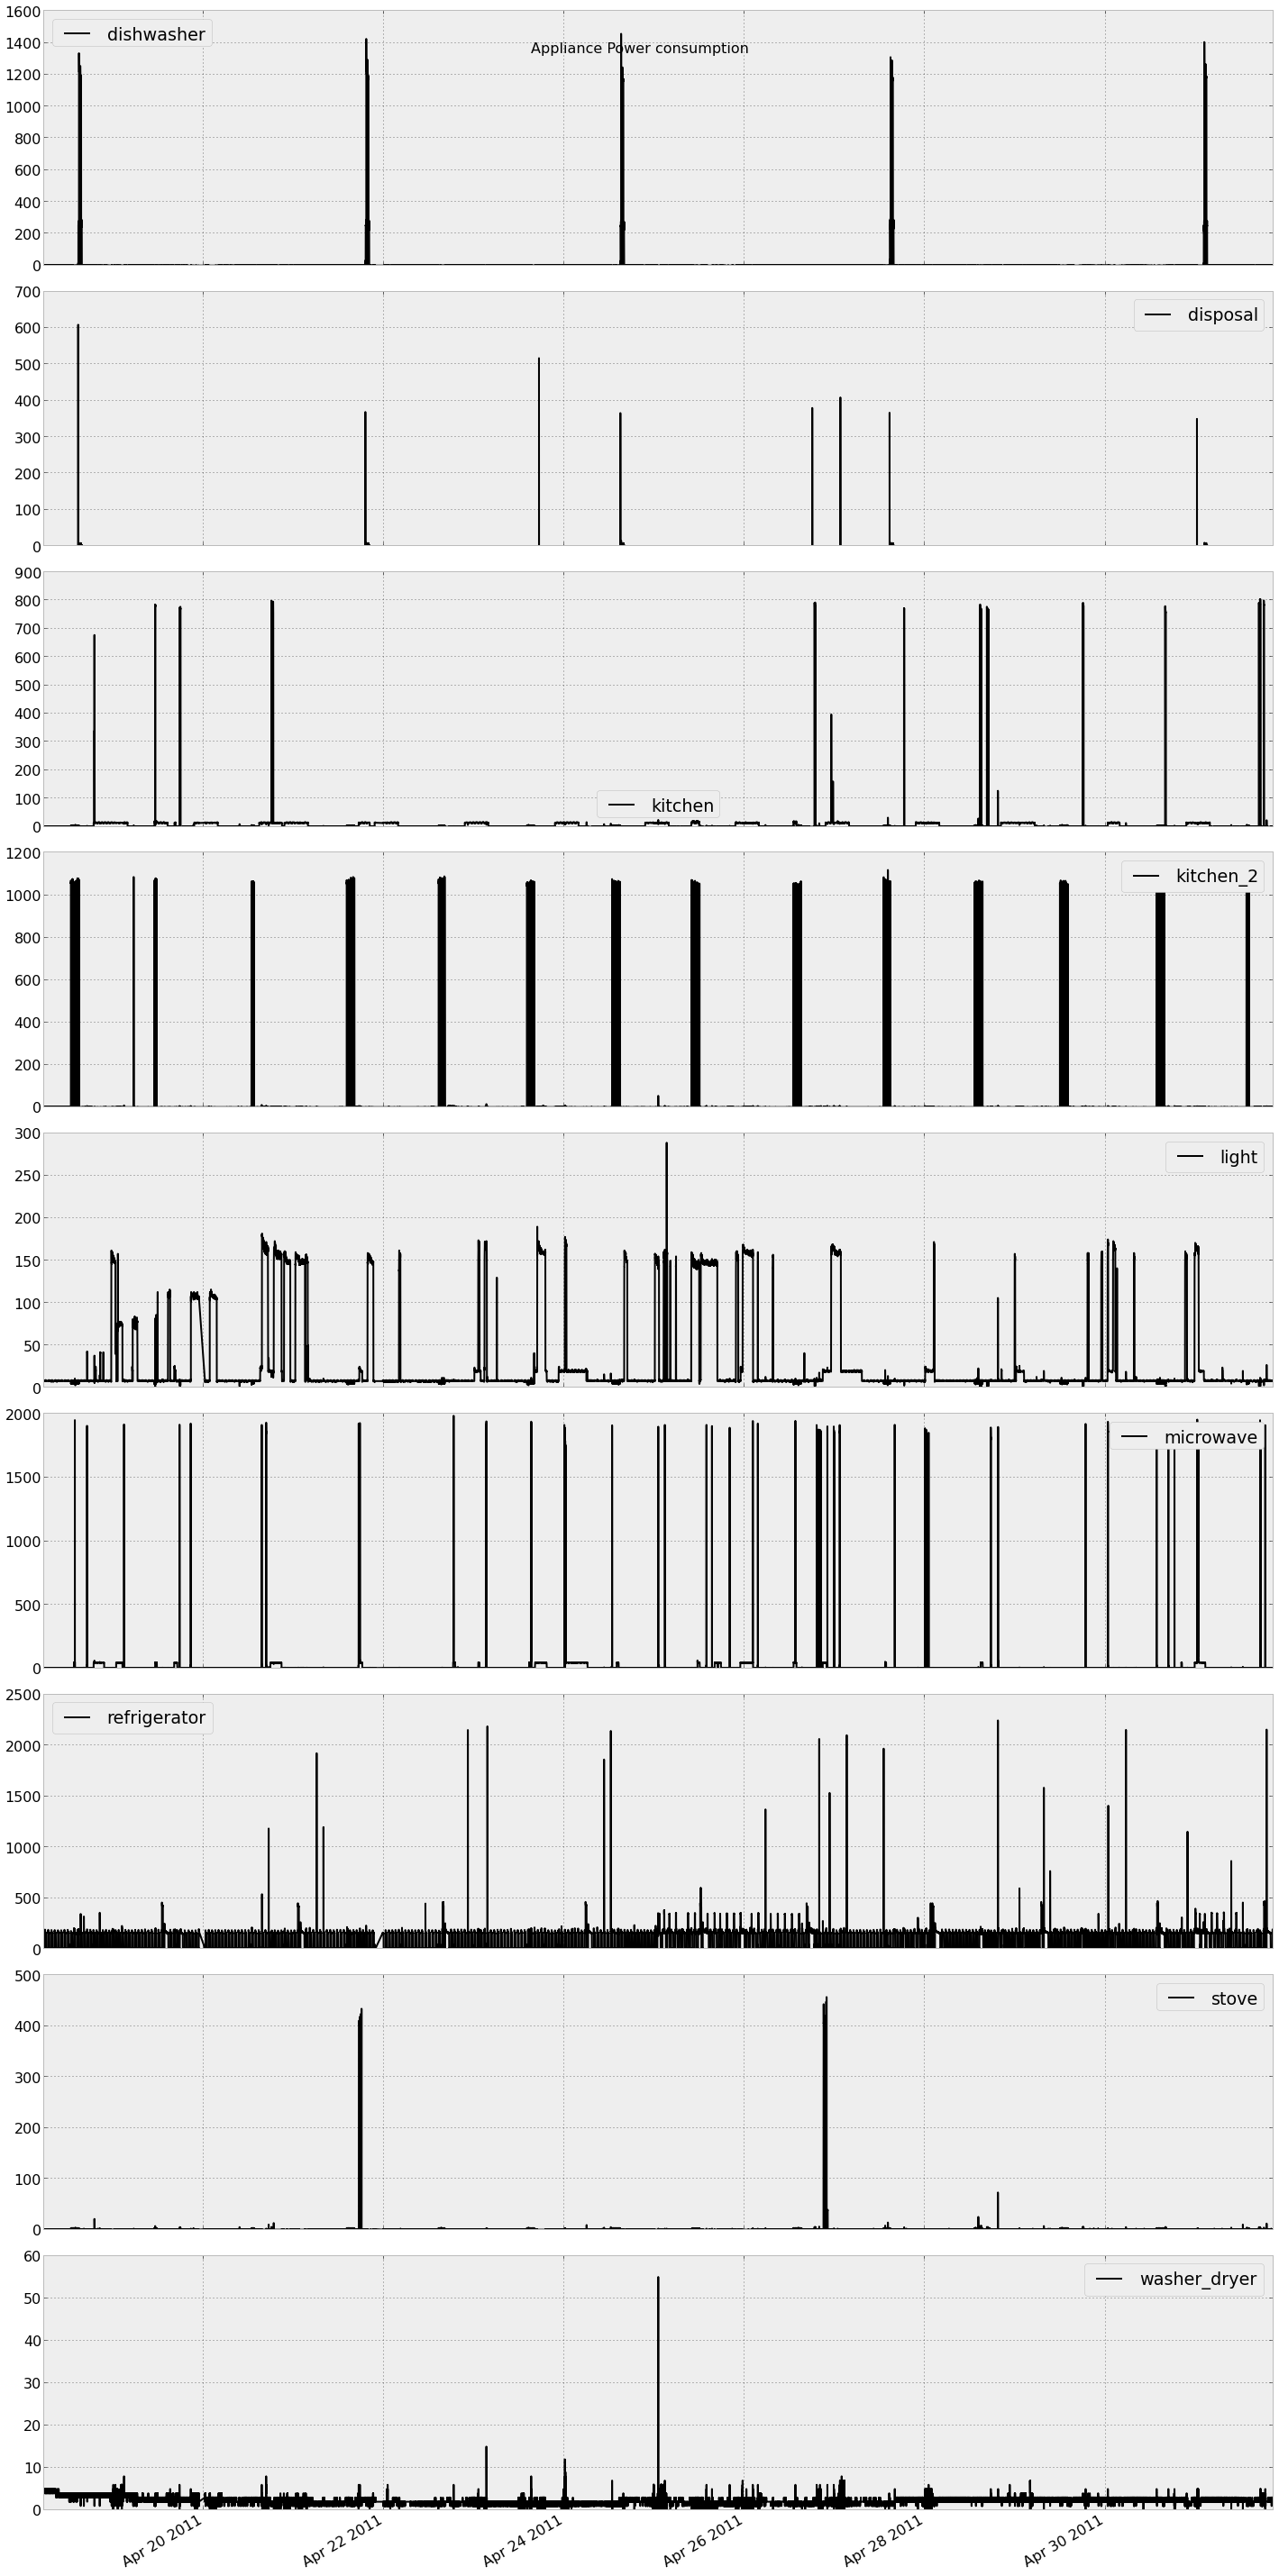
\includegraphics[width=0.7\textwidth]{REDD_House2_Analysis_files/REDD_House2_Analysis_fig_07.png}
\par
\end{center}
\end{codeoutput}
\end{codecell}
\subsection{Assigning loads to different mains circuits}
Since there are two mains in the home we need to break down the
individual appliance into different mains. Clearly,

\begin{itemize}
\item
  Kitchen\_2 belongs to Mains1
\item
  Kitchen belongs to Mains1
\item
  Refrigerator belongs to Mains 2
\end{itemize}

Beyond this it is difficult to visually find the mains corresponding to
different appliances. We thus decide to iteratively remove the known
components. It must be noted that Mains is at 1 Hz and appliance are at
lower resolution. Thus we need to align the two. This we do by aligning
higher frequency mains to lower resolution appliance resolution. Thus,
we downsample both the mains and all the appliances to a minute
resolution, taking mean of the values contained within the minute.

\begin{codecell}
\begin{codeinput}
\begin{lstlisting}
df_appliances_minute=df_appliances.resample('1Min',how='mean')
pd.set_option('display.precision', 2)
print df_appliances_minute.describe().to_string()
\end{lstlisting}
\end{codeinput}
\begin{codeoutput}
\begin{verbatim}
dishwasher  disposal  kitchen  kitchen_2    light  microwave  refrigerator    stove  washer_dryer
count     19398.0   19398.0  19398.0    19398.0  19398.0    19398.0       19398.0  19398.0       19398.0
mean          9.3       0.1      6.1       10.6     26.9       14.4          79.6      1.5           2.2
std          96.5       1.6     35.0       74.5     46.1       89.7          85.5     18.1           0.6
min           0.0       0.0      0.0        0.0      2.0        1.6           1.6      0.0           0.0
25%           0.0       0.0      0.0        1.0      8.0        4.1           6.1      0.1           2.0
50%           0.1       0.0      0.4        1.0      8.6        4.6           7.0      0.5           2.0
75%           0.1       0.0     13.0        1.0      9.0        5.0         160.8      0.9           2.2
max        1255.6     115.8    794.6     1071.8    185.4     1926.0         598.2    411.0           8.8
\end{verbatim}
\end{codeoutput}
\end{codecell}
As a sanity check, we confirm that 19400 minutes correspond to about 14
days, thus our resampling was correct. We next align mains and appliance
time series.

\begin{codecell}
\begin{codeinput}
\begin{lstlisting}
df_mains_minute=df_mains.resample('1Min',how='mean')
df_mains_minute.describe()
print df_mains_minute.index
print np.where(df_mains_minute.index==df_appliances_minute.index[0])
df_mains_minute=df_mains_minute[236:]

print df_mains_minute.index
df_mains_minute.describe()
\end{lstlisting}
\end{codeinput}
\begin{codeoutput}
\begin{verbatim}
<class 'pandas.tseries.index.DatetimeIndex'>
[2011-04-18 01:45:00, ..., 2011-05-01 20:38:00]
Length: 19854, Freq: T, Timezone: None
(array([236]),)
<class 'pandas.tseries.index.DatetimeIndex'>
[2011-04-18 05:41:00, ..., 2011-05-01 20:38:00]
Length: 19618, Freq: T, Timezone: None
\end{verbatim}
\begin{verbatim}
       Mains_1_Power  Mains_2_Power
count        19397.0        19397.0
mean            43.5          187.7
std            130.4          204.1
min             13.4           21.4
25%             14.9           22.5
50%             15.1          214.4
75%             33.7          259.1
max           1312.0         2612.5
\end{verbatim}
\end{codeoutput}
\end{codecell}
We now plot the lower resolution mains 1 and iteratively attempt to take
out appliances.

\begin{codecell}
\begin{codeinput}
\begin{lstlisting}
figsize(20,15)
ax=df_mains_minute.Mains_1_Power.plot(title='1 min downsampled Power Mains 1');
ax.set_ylabel("Power (W)");
\end{lstlisting}
\end{codeinput}
\begin{codeoutput}
\begin{center}
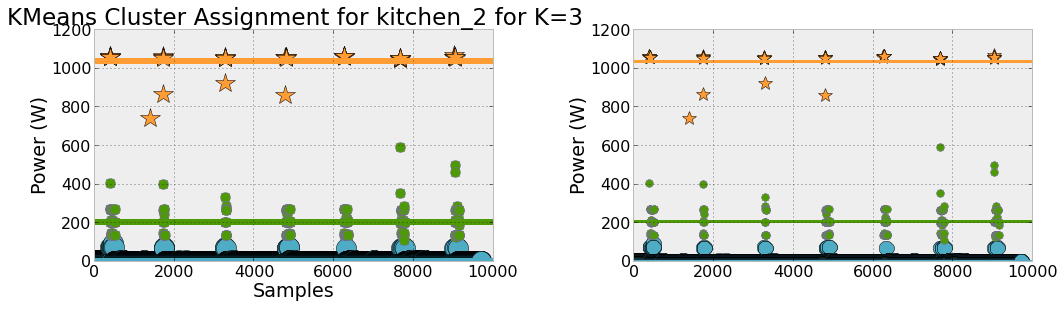
\includegraphics[width=0.7\textwidth]{REDD_House2_Analysis_files/REDD_House2_Analysis_fig_08.png}
\par
\end{center}
\end{codeoutput}
\end{codecell}
Removing kitchen\_2 from Mains 1

\begin{codecell}
\begin{codeinput}
\begin{lstlisting}
temp_1=df_mains_minute.Mains_1_Power-df_appliances_minute.kitchen_2
temp_1[temp_1<0.0]=0.0
\end{lstlisting}
\end{codeinput}
\end{codecell}
\begin{codecell}
\begin{codeinput}
\begin{lstlisting}
df_mains_minute_minus_kitchen_2=df_mains_minute.copy()
df_mains_minute_minus_kitchen_2.Mains_1_Power=temp_1
print "Before\n\n",df_mains_minute.describe()
print "\nAfter\n\n",df_mains_minute_minus_kitchen_2.describe()
ax=df_mains_minute_minus_kitchen_2.Mains_1_Power.plot(title='Mains 1 Power Minus Kitchen 2')
ax.set_ylabel('Power');
\end{lstlisting}
\end{codeinput}
\begin{codeoutput}
\begin{verbatim}
Before

       Mains_1_Power  Mains_2_Power
count        19397.0        19397.0
mean            43.5          187.7
std            130.4          204.1
min             13.4           21.4
25%             14.9           22.5
50%             15.1          214.4
75%             33.7          259.1
max           1312.0         2612.5

After

       Mains_1_Power  Mains_2_Power
count        19395.0        19397.0
mean            33.2          187.7
std            107.0          204.1
min              0.0           21.4
25%             13.7           22.5
50%             14.1          214.4
75%             32.4          259.1
max           1312.0         2612.5
\end{verbatim}
\begin{center}
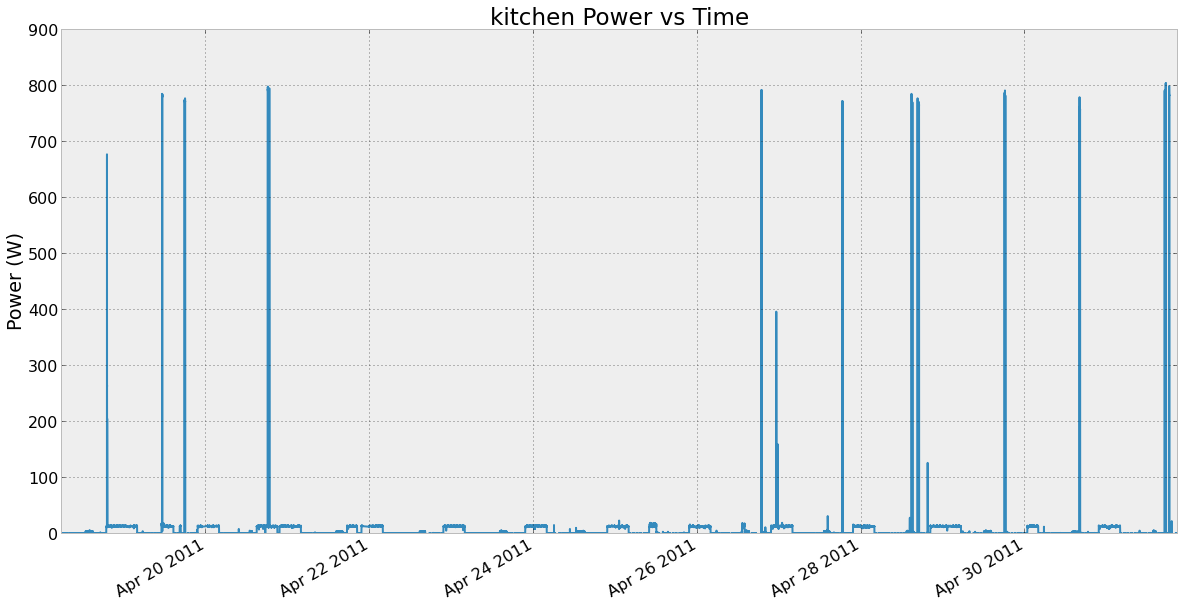
\includegraphics[width=0.7\textwidth]{REDD_House2_Analysis_files/REDD_House2_Analysis_fig_09.png}
\par
\end{center}
\end{codeoutput}
\end{codecell}
Now removing Kitchen 1 from mains 1

\begin{codecell}
\begin{codeinput}
\begin{lstlisting}
temp_2=df_mains_minute_minus_kitchen_2.Mains_1_Power-df_appliances_minute.kitchen
temp_2[temp_2<0.0]=0.0
\end{lstlisting}
\end{codeinput}
\end{codecell}
\begin{codecell}
\begin{codeinput}
\begin{lstlisting}
df_mains_minute_minus_kitchen_2_1=df_mains_minute_minus_kitchen_2.copy()
df_mains_minute_minus_kitchen_2_1.Mains_1_Power=temp_2
print "Before\n\n",df_mains_minute_minus_kitchen_2.describe()
print "\nAfter\n\n",df_mains_minute_minus_kitchen_2_1.describe()
ax=df_mains_minute_minus_kitchen_2_1.Mains_1_Power.plot(title='Mains 1 Power Minus Kitchen 2 and Kitchen 1')
ax.set_ylabel('Power');
\end{lstlisting}
\end{codeinput}
\begin{codeoutput}
\begin{verbatim}
Before

       Mains_1_Power  Mains_2_Power
count        19395.0        19397.0
mean            33.2          187.7
std            107.0          204.1
min              0.0           21.4
25%             13.7           22.5
50%             14.1          214.4
75%             32.4          259.1
max           1312.0         2612.5

After

       Mains_1_Power  Mains_2_Power
count        19395.0        19397.0
mean            27.1          187.7
std            100.7          204.1
min              0.0           21.4
25%             13.5           22.5
50%             13.7          214.4
75%             18.6          259.1
max           1299.0         2612.5
\end{verbatim}
\begin{center}
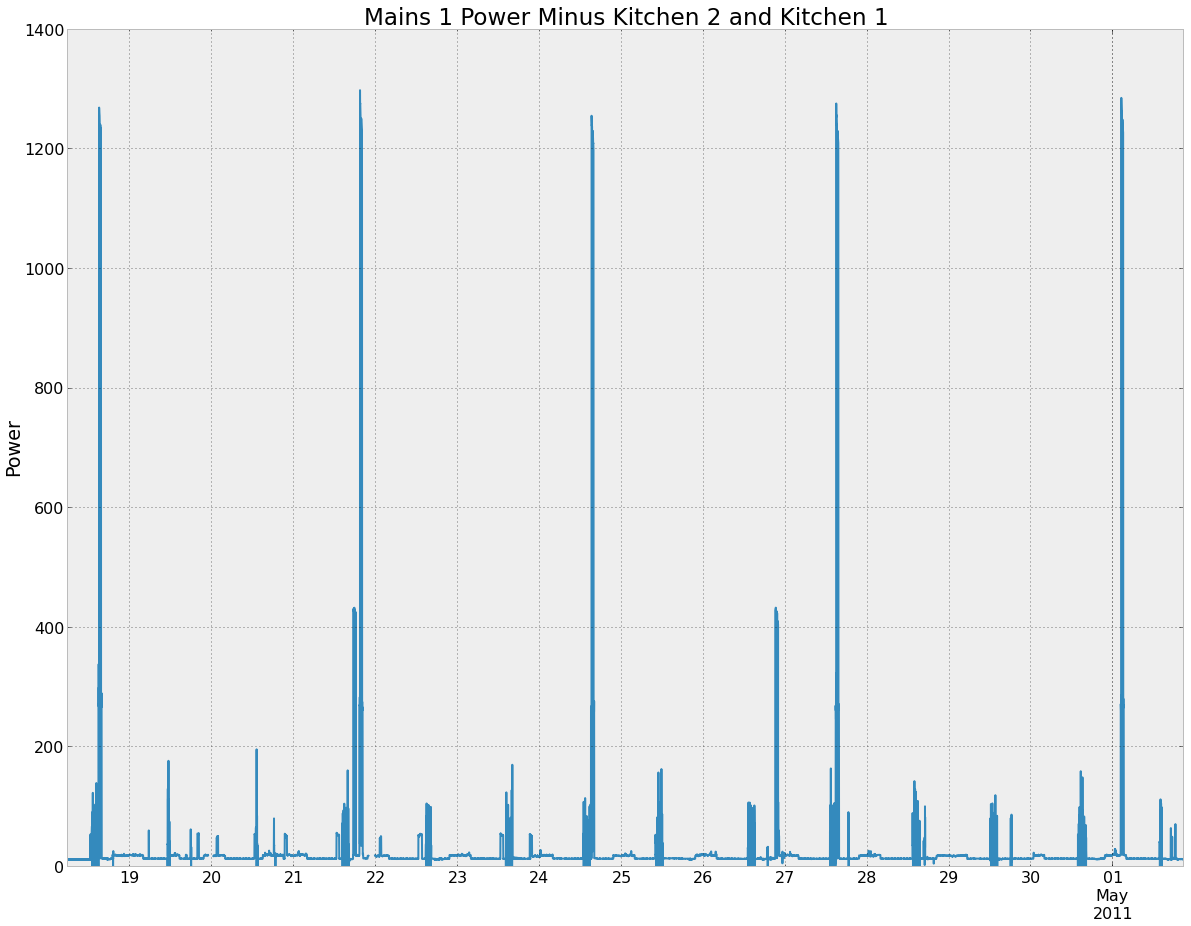
\includegraphics[width=0.7\textwidth]{REDD_House2_Analysis_files/REDD_House2_Analysis_fig_10.png}
\par
\end{center}
\end{codeoutput}
\end{codecell}
Now we observe that Dishwasher was used every 3rd day starting from 19th
and power consumption was about 1200+ W. Thus, we next remove the
dishwasher component from mains 1

\begin{codecell}
\begin{codeinput}
\begin{lstlisting}
temp_3=df_mains_minute_minus_kitchen_2_1.Mains_1_Power-df_appliances_minute.dishwasher
temp_3[temp_3<0.0]=0.0
\end{lstlisting}
\end{codeinput}
\end{codecell}
\begin{codecell}
\begin{codeinput}
\begin{lstlisting}
df_mains_minute_minus_kitchen_dishwasher=df_mains_minute_minus_kitchen_2_1.copy()
df_mains_minute_minus_kitchen_dishwasher.Mains_1_Power=temp_3
print "Before\n\n",df_mains_minute_minus_kitchen_2_1.describe()
print "\nAfter\n\n",df_mains_minute_minus_kitchen_dishwasher.describe()
ax=df_mains_minute_minus_kitchen_dishwasher.Mains_1_Power.plot(title='Mains 1 Power Minus Kitchen and Dishwasher')
ax.set_ylabel('Power');
\end{lstlisting}
\end{codeinput}
\begin{codeoutput}
\begin{verbatim}
Before

       Mains_1_Power  Mains_2_Power
count        19395.0        19397.0
mean            27.1          187.7
std            100.7          204.1
min              0.0           21.4
25%             13.5           22.5
50%             13.7          214.4
75%             18.6          259.1
max           1299.0         2612.5

After

       Mains_1_Power  Mains_2_Power
count        19395.0        19397.0
mean            17.8          187.7
std             20.9          204.1
min              0.0           21.4
25%             13.5           22.5
50%             13.7          214.4
75%             18.5          259.1
max            433.4         2612.5
\end{verbatim}
\begin{center}
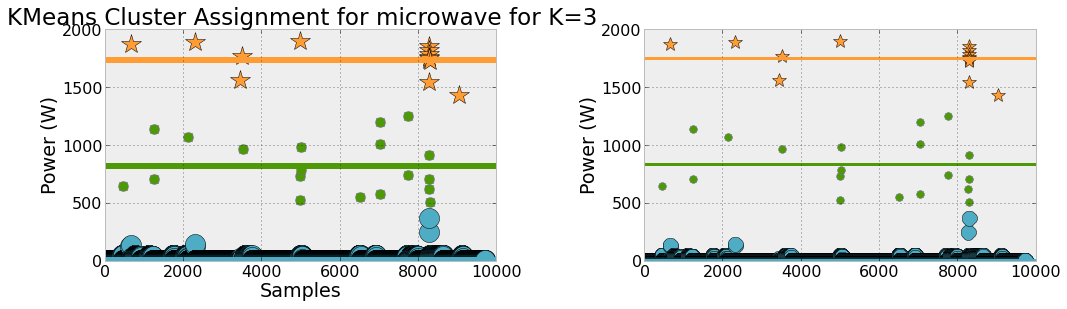
\includegraphics[width=0.7\textwidth]{REDD_House2_Analysis_files/REDD_House2_Analysis_fig_11.png}
\par
\end{center}
\end{codeoutput}
\end{codecell}
Removing stove from Mains 1

\begin{codecell}
\begin{codeinput}
\begin{lstlisting}
temp_4=df_mains_minute_minus_kitchen_dishwasher.Mains_1_Power-df_appliances_minute.stove
temp_4[temp_4<0.0]=0.0
\end{lstlisting}
\end{codeinput}
\end{codecell}
\begin{codecell}
\begin{codeinput}
\begin{lstlisting}
df_mains_minute_minus_kitchen_dishwasher_stove=df_mains_minute_minus_kitchen_dishwasher.copy()
df_mains_minute_minus_kitchen_dishwasher_stove.Mains_1_Power=temp_4
print "Before\n\n",df_mains_minute_minus_kitchen_dishwasher.describe()
print "\nAfter\n\n",df_mains_minute_minus_kitchen_dishwasher_stove.describe()
ax=df_mains_minute_minus_kitchen_dishwasher_stove.Mains_1_Power.plot(title='Mains 1 Power Minus Kitchen, Dishwasher and Stove')
ax.set_ylabel('Power');
\end{lstlisting}
\end{codeinput}
\begin{codeoutput}
\begin{verbatim}
Before

       Mains_1_Power  Mains_2_Power
count        19395.0        19397.0
mean            17.8          187.7
std             20.9          204.1
min              0.0           21.4
25%             13.5           22.5
50%             13.7          214.4
75%             18.5          259.1
max            433.4         2612.5

After

       Mains_1_Power  Mains_2_Power
count        19395.0        19397.0
mean            16.3          187.7
std              9.9          204.1
min              0.0           21.4
25%             12.7           22.5
50%             13.4          214.4
75%             17.7          259.1
max            196.0         2612.5
\end{verbatim}
\begin{center}
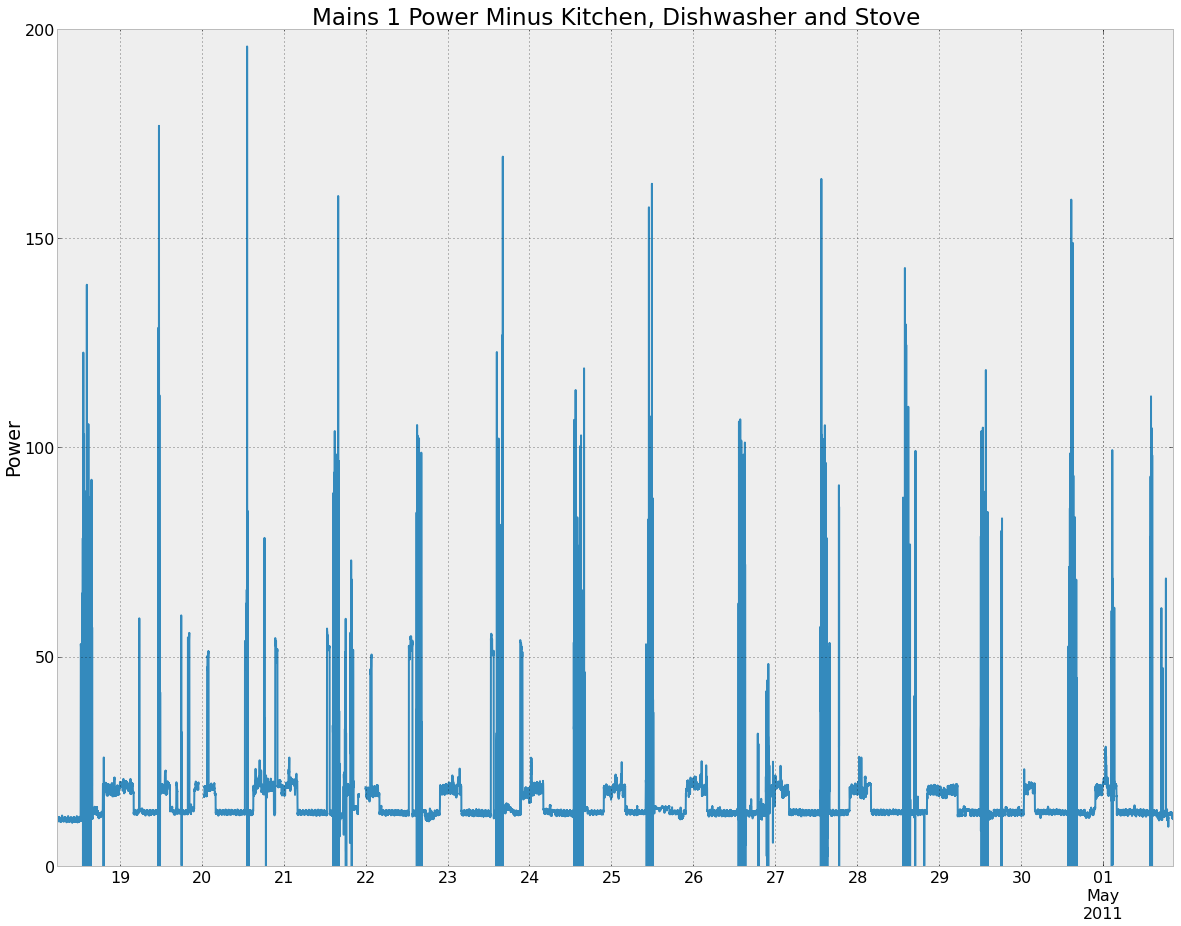
\includegraphics[width=0.7\textwidth]{REDD_House2_Analysis_files/REDD_House2_Analysis_fig_12.png}
\par
\end{center}
\end{codeoutput}
\end{codecell}
We next observe that none of the other appliance can be extracted
visually from Mains 1. So we start removing appliances iteratively from
Mains 2. \textbf{From the next plot we can see that there is a slight
difference in power seen by the mains and the appliance level monitor,
hence there seems to be a need to do this calibration to ensure that we
have better results. Moreover, this is an aspect i think no one has yet
highlighted in their work}.

\begin{codecell}
\begin{codeinput}
\begin{lstlisting}
temp_5=df_mains_minute_minus_kitchen_dishwasher_stove.Mains_2_Power-df_appliances_minute.refrigerator
temp_5[temp_5<0.0]=0.0
plt.subplot(3,1,1)
df_appliances_minute.refrigerator.plot(title='Refrigerator')
plt.subplot(3,1,2)
df_mains_minute.Mains_2_Power.plot(title='Mains 2')
plt.subplot(3,1,3)
temp_5.plot(title='Mains 2 after removing refrigerator');
plt.tight_layout()
\end{lstlisting}
\end{codeinput}
\begin{codeoutput}
\begin{center}
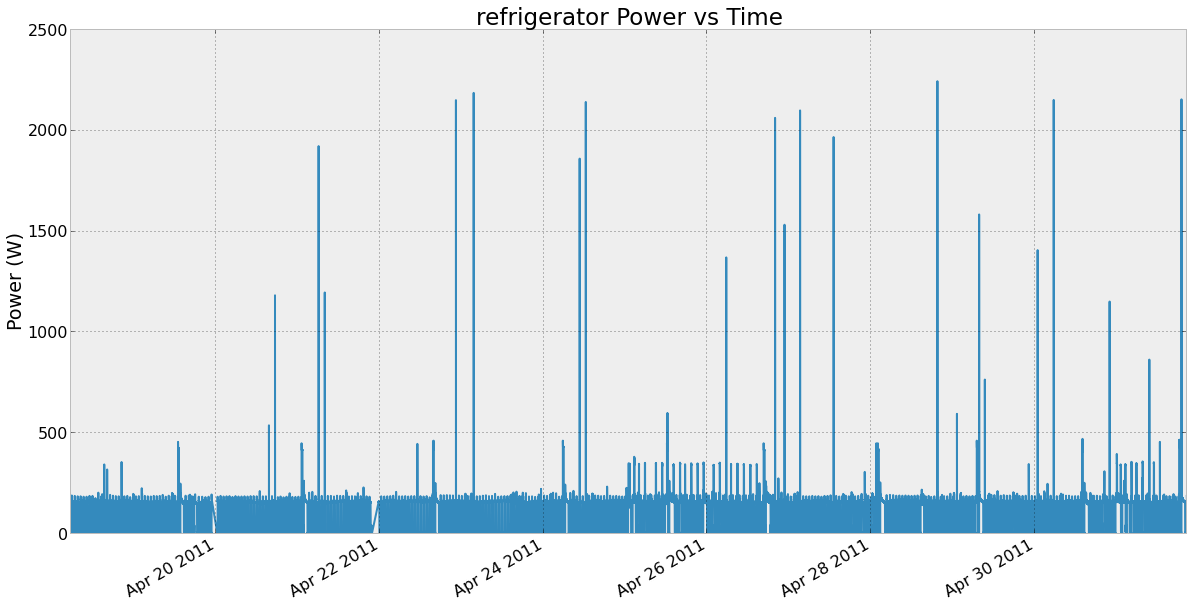
\includegraphics[width=0.7\textwidth]{REDD_House2_Analysis_files/REDD_House2_Analysis_fig_13.png}
\par
\end{center}
\end{codeoutput}
\end{codecell}
\begin{codecell}
\begin{codeinput}
\begin{lstlisting}
df_mains_minute_minus_kitchen_dishwasher_stove_ref=df_mains_minute_minus_kitchen_dishwasher_stove.copy()
df_mains_minute_minus_kitchen_dishwasher_stove_ref.Mains_2_Power=temp_5
print "Before\n\n",df_mains_minute_minus_kitchen_dishwasher_stove.describe()
print "\nAfter\n\n",df_mains_minute_minus_kitchen_dishwasher_stove_ref.describe()
ax=df_mains_minute_minus_kitchen_dishwasher_stove_ref.Mains_2_Power.plot(title='Mains 2 Power Minus Refrigerator')
ax.set_ylabel('Power');
\end{lstlisting}
\end{codeinput}
\begin{codeoutput}
\begin{verbatim}
Before

       Mains_1_Power  Mains_2_Power
count        19395.0        19397.0
mean            16.3          187.7
std              9.9          204.1
min              0.0           21.4
25%             12.7           22.5
50%             13.4          214.4
75%             17.7          259.1
max            196.0         2612.5

After

       Mains_1_Power  Mains_2_Power
count        19395.0        19395.0
mean            16.3          108.1
std              9.9          168.1
min              0.0            0.0
25%             12.7           16.3
50%             13.4           89.3
75%             17.7           97.5
max            196.0         2448.5
\end{verbatim}
\begin{center}
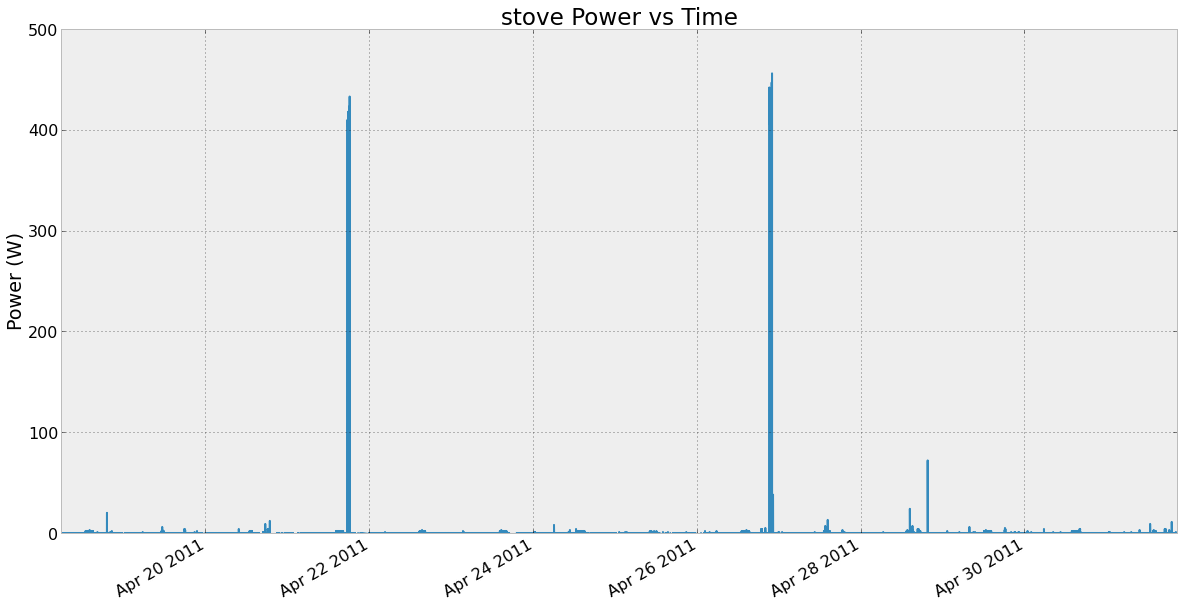
\includegraphics[width=0.7\textwidth]{REDD_House2_Analysis_files/REDD_House2_Analysis_fig_14.png}
\par
\end{center}
\end{codeoutput}
\end{codecell}
Since microwave is taking more power than residual power in Mains 1, it
has to belong to Mains 2. Next, removing Microwave from Mains 2.

\begin{codecell}
\begin{codeinput}
\begin{lstlisting}
temp_6=df_mains_minute_minus_kitchen_dishwasher_stove_ref.Mains_2_Power-df_appliances_minute.microwave
temp_6[temp_6<0.0]=0.0
\end{lstlisting}
\end{codeinput}
\end{codecell}
\begin{codecell}
\begin{codeinput}
\begin{lstlisting}
df_mains_minute_minus_kitchen_dishwasher_stove_ref_micro=df_mains_minute_minus_kitchen_dishwasher_stove_ref.copy()
df_mains_minute_minus_kitchen_dishwasher_stove_ref_micro.Mains_2_Power=temp_6
print "Before\n\n",df_mains_minute_minus_kitchen_dishwasher_stove_ref.describe()
print "\nAfter\n\n",df_mains_minute_minus_kitchen_dishwasher_stove_ref_micro.describe()
ax=df_mains_minute_minus_kitchen_dishwasher_stove_ref_micro.Mains_2_Power.plot(title='Mains 2 Power Minus Refrigerator and Micro')
ax.set_ylabel('Power');
\end{lstlisting}
\end{codeinput}
\begin{codeoutput}
\begin{verbatim}
Before

       Mains_1_Power  Mains_2_Power
count        19395.0        19395.0
mean            16.3          108.1
std              9.9          168.1
min              0.0            0.0
25%             12.7           16.3
50%             13.4           89.3
75%             17.7           97.5
max            196.0         2448.5

After

       Mains_1_Power  Mains_2_Power
count        19395.0        19395.0
mean            16.3           93.6
std              9.9          136.0
min              0.0            0.0
25%             12.7           12.2
50%             13.4           80.0
75%             17.7           91.6
max            196.0         1177.5
\end{verbatim}
\begin{center}
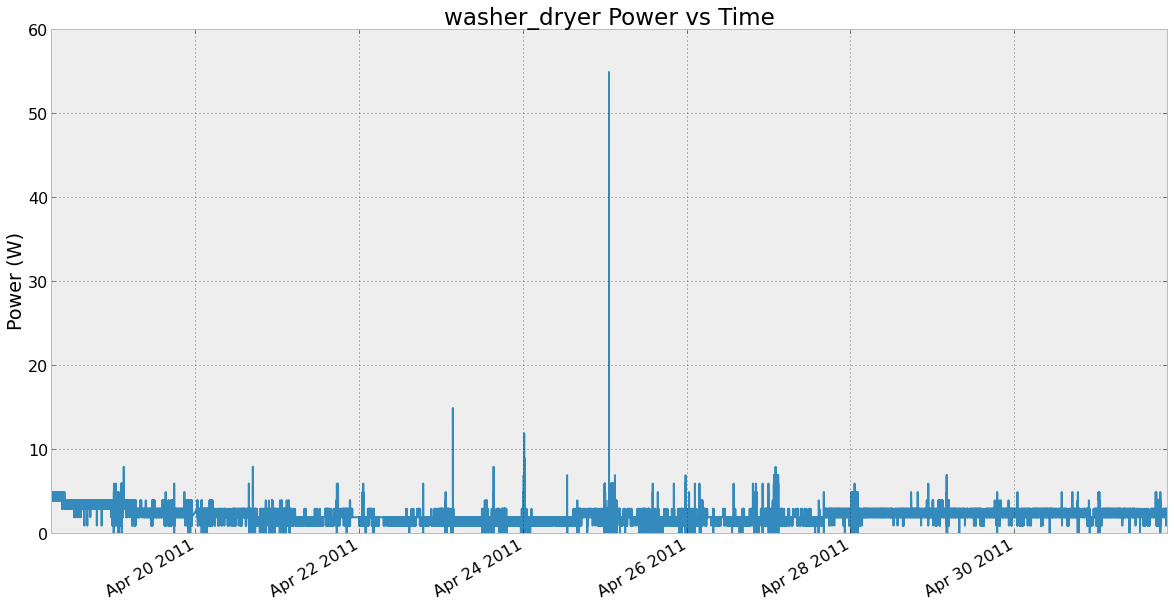
\includegraphics[width=0.7\textwidth]{REDD_House2_Analysis_files/REDD_House2_Analysis_fig_15.png}
\par
\end{center}
\end{codeoutput}
\end{codecell}
An interesting thing to note is the correlation between
\textbf{Disposal} and \textbf{Dishwasher} both of which occur on the
same days. Next, we iteratively start extracting out appliances from
Mains 2.

Removing lighting from Mains 2.

\begin{codecell}
\begin{codeinput}
\begin{lstlisting}
temp_7=df_mains_minute_minus_kitchen_dishwasher_stove_ref_micro.Mains_2_Power-df_appliances_minute.light
temp_7[temp_7<0.0]=0.0
\end{lstlisting}
\end{codeinput}
\end{codecell}
\begin{codecell}
\begin{codeinput}
\begin{lstlisting}
df_mains_minute_minus_kitchen_dishwasher_stove_ref_micro_light=df_mains_minute_minus_kitchen_dishwasher_stove_ref_micro.copy()
df_mains_minute_minus_kitchen_dishwasher_stove_ref_micro_light.Mains_2_Power=temp_7
print "Before\n\n",df_mains_minute_minus_kitchen_dishwasher_stove_ref_micro.describe()
print "\nAfter\n\n",df_mains_minute_minus_kitchen_dishwasher_stove_ref_micro_light.describe()
ax=df_mains_minute_minus_kitchen_dishwasher_stove_ref_micro_light.Mains_2_Power.plot(title='Mains 2 Power Minus Refrigerator, Micro and Lighting')
ax.set_ylabel('Power');
\end{lstlisting}
\end{codeinput}
\begin{codeoutput}
\begin{verbatim}
Before

       Mains_1_Power  Mains_2_Power
count        19395.0        19395.0
mean            16.3           93.6
std              9.9          136.0
min              0.0            0.0
25%             12.7           12.2
50%             13.4           80.0
75%             17.7           91.6
max            196.0         1177.5

After

       Mains_1_Power  Mains_2_Power
count        19395.0        19395.0
mean            16.3           66.7
std              9.9          120.2
min              0.0            0.0
25%             12.7            4.2
50%             13.4           45.7
75%             17.7           80.3
max            196.0         1017.3
\end{verbatim}
\begin{center}
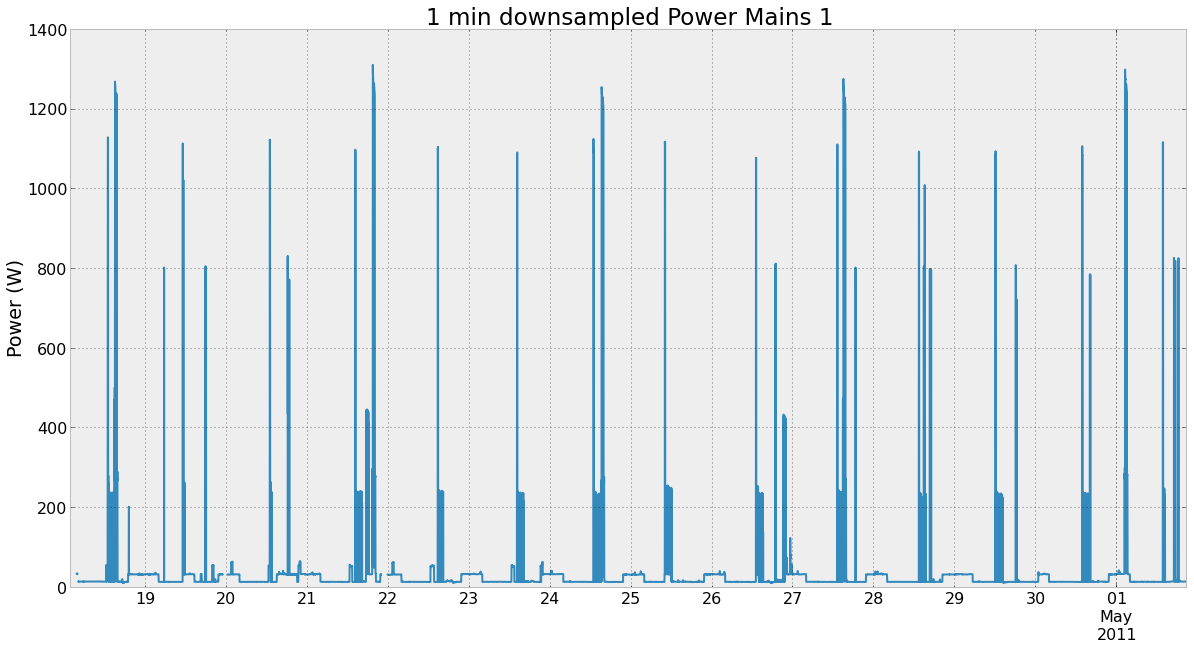
\includegraphics[width=0.7\textwidth]{REDD_House2_Analysis_files/REDD_House2_Analysis_fig_16.png}
\par
\end{center}
\end{codeoutput}
\end{codecell}
Thus, we can see that both for Mains 1 and Mains 2 there is still a lot
of unaccounted power. This is due to mis calibration between the
appliance level loads and also due to absence of complete information.
This is an important aspect to address. Next, we draw the boxplot
showing unaccounted power.

\begin{codecell}
\begin{codeinput}
\begin{lstlisting}
plt.figure()
plt.title("Unaccounted Power")
plt.ylabel("Power (W)")
df_mains_minute_minus_kitchen_dishwasher_stove_ref_micro_light.boxplot();
\end{lstlisting}
\end{codeinput}
\begin{codeoutput}
\begin{center}
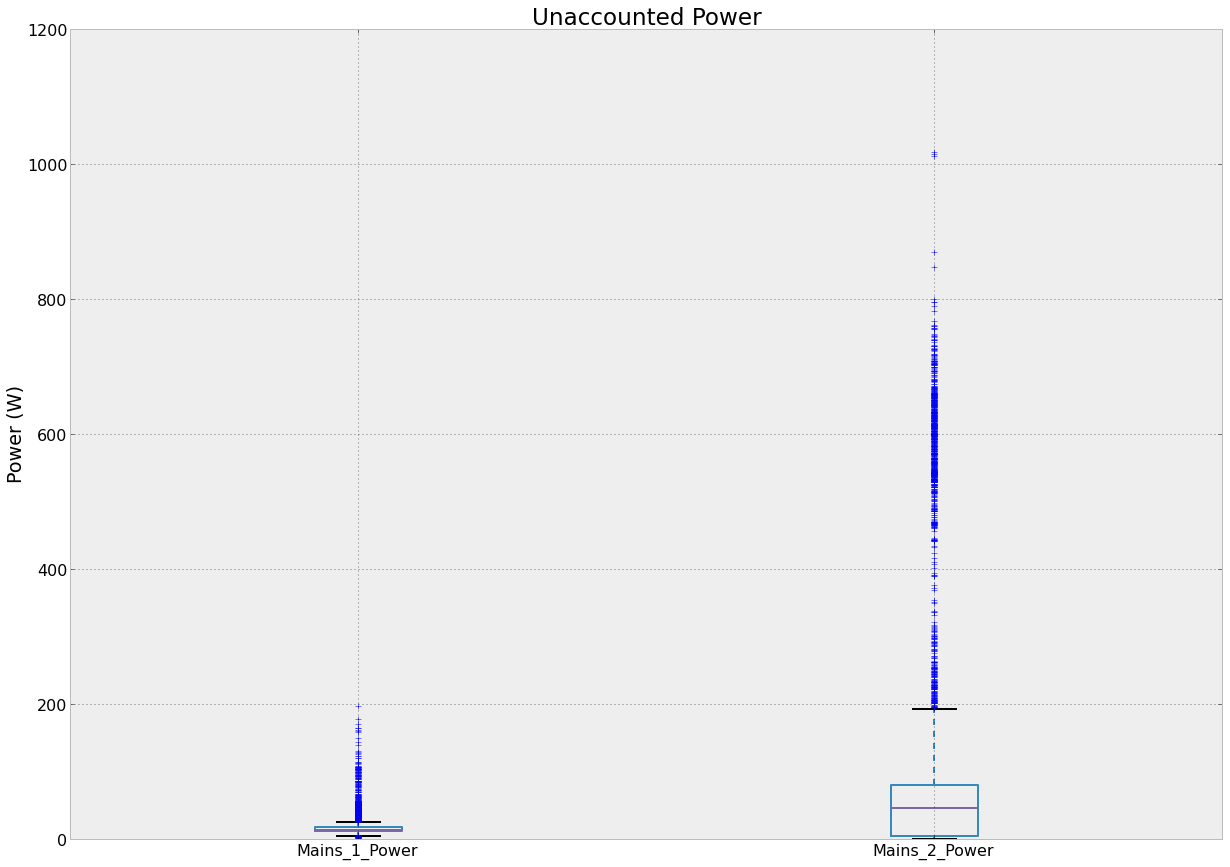
\includegraphics[width=0.7\textwidth]{REDD_House2_Analysis_files/REDD_House2_Analysis_fig_17.png}
\par
\end{center}
\end{codeoutput}
\end{codecell}
\subsubsection{Breakdown by appliance}
Mains 1

\begin{codecell}
\begin{codeinput}
\begin{lstlisting}
labels = 'Kitchen 1', 'Kitchen 2', 'Dishwasher', 'Stove','Unaccounted'
kitchen_mean,kitchen_2_mean,dishwasher_mean,stove_mean=df_appliances_minute.kitchen.mean(),\
df_appliances_minute.kitchen_2.mean(),df_appliances_minute.dishwasher.mean(),df_appliances_minute.stove.mean()
unaccounted_mean=df_mains_minute.Mains_1_Power.mean()-(kitchen_mean+kitchen_2_mean+dishwasher_mean+stove_mean)

fracs = [kitchen_mean,kitchen_2_mean,dishwasher_mean,stove_mean,unaccounted_mean]
explode=(0, 0, 0, 0,0)
plt.figsize(7,7)
plt.title('Power Breakdown by appliance Mains 1');
plt.pie(fracs, explode=explode, labels=labels,autopct='%1.1f%%', shadow=True);              

\end{lstlisting}
\end{codeinput}
\begin{codeoutput}
\begin{center}
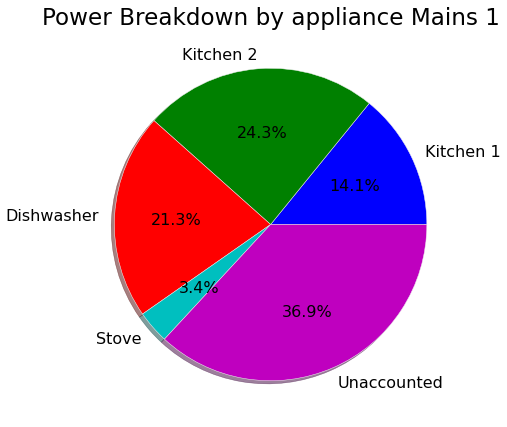
\includegraphics[width=0.7\textwidth]{REDD_House2_Analysis_files/REDD_House2_Analysis_fig_18.png}
\par
\end{center}
\end{codeoutput}
\end{codecell}
\begin{codecell}
\begin{codeinput}
\begin{lstlisting}
labels = 'Refrigerator', 'Microwave', 'Lighting','Unaccounted Power'
refrigerator_mean,microwave_mean,lighting_mean=df_appliances_minute.refrigerator.mean(),\
df_appliances_minute.microwave.mean(),df_appliances_minute.light.mean()
unaccounted_mean=df_mains_minute.Mains_2_Power.mean()-(refrigerator_mean+microwave_mean+lighting_mean)

fracs = [refrigerator_mean,microwave_mean,lighting_mean,unaccounted_mean]
explode=(0, 0, 0,0)
plt.figsize(7,7)
plt.title('Power Breakdown by appliance Mains 2');
plt.pie(fracs, explode=explode, labels=labels,autopct='%1.1f%%', shadow=True); 
\end{lstlisting}
\end{codeinput}
\begin{codeoutput}
\begin{center}
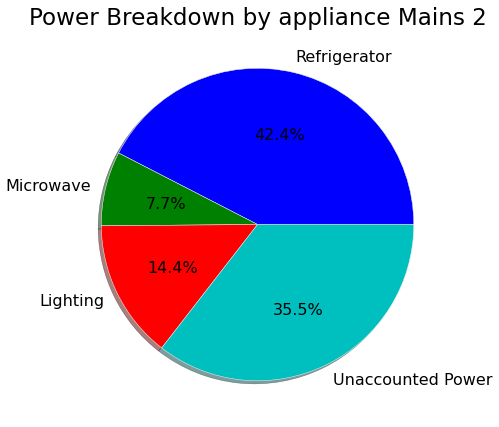
\includegraphics[width=0.7\textwidth]{REDD_House2_Analysis_files/REDD_House2_Analysis_fig_19.png}
\par
\end{center}
\end{codeoutput}
\end{codecell}
Thus, we can see that in both the mains circuits about 1/3 of total
power cannot be attributed to any appliance.

\begin{codecell}
\begin{codeinput}
\begin{lstlisting}
labels = 'Mains 1','Mains 2'

fracs = [df_mains_minute.Mains_1_Power.mean(),df_mains_minute.Mains_2_Power.mean()]
explode=(0, 0)
plt.figsize(7,7)
plt.title('Power Breakdown by Mains');
plt.pie(fracs, explode=explode, labels=labels,autopct='%1.1f%%', shadow=True); 
\end{lstlisting}
\end{codeinput}
\begin{codeoutput}
\begin{center}
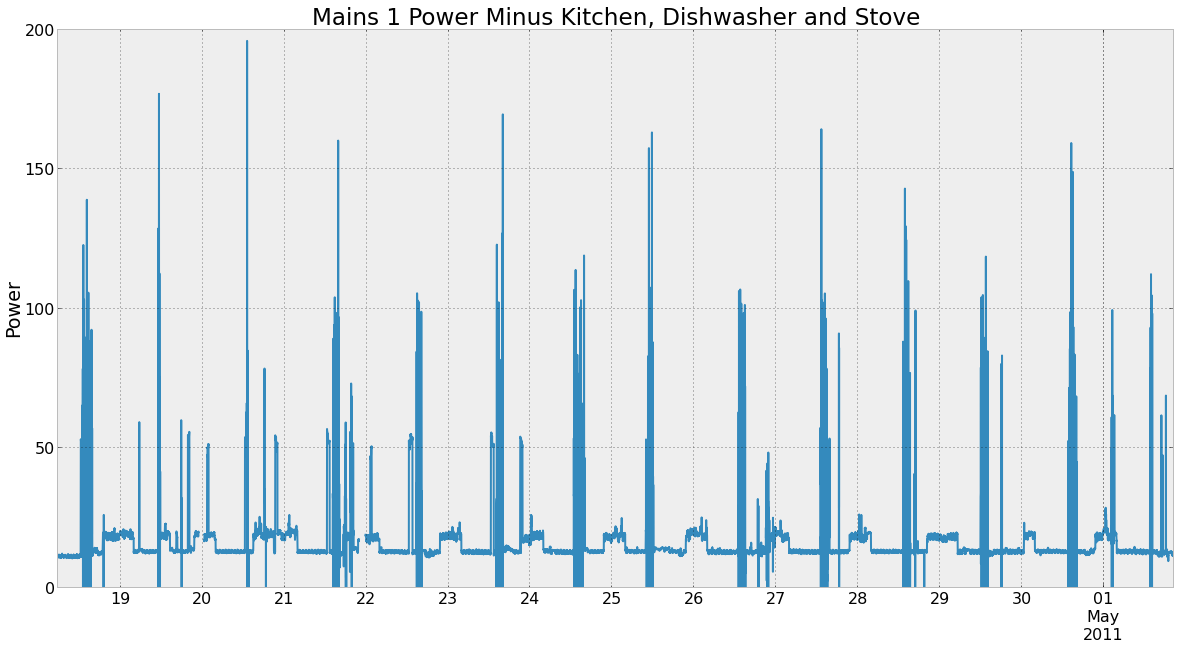
\includegraphics[width=0.7\textwidth]{REDD_House2_Analysis_files/REDD_House2_Analysis_fig_20.png}
\par
\end{center}
\end{codeoutput}
\end{codecell}
Remaining load is unaccounted for in the analysis. We now have 2
options:

\begin{itemize}
\item
  To continue with this data as such and not process further
\item
  To filter out data about which not information has been provided
\end{itemize}

Option 1 is more realistic and Option 2 is more ideal. We shall be
considering the ideal case through the remaining analysis. Thus, we need
to filter out the remaining data.

\begin{codecell}
\begin{codeinput}
\begin{lstlisting}
filtered_mains_1_power=df_appliances_minute.kitchen+df_appliances_minute.kitchen_2+df_appliances_minute.stove+\
df_appliances_minute.dishwasher

filtered_mains_2_power=df_appliances_minute.refrigerator+df_appliances_minute.light+df_appliances_minute.microwave
\end{lstlisting}
\end{codeinput}
\end{codecell}
\begin{codecell}
\begin{codeinput}
\begin{lstlisting}
df_filtered_mains=pd.DataFrame({'Mains_1_Power':filtered_mains_1_power,'Mains_2_Power':filtered_mains_2_power},\
index=df_mains_minute_minus_kitchen_dishwasher_stove_ref_micro_light.index)
\end{lstlisting}
\end{codeinput}
\end{codecell}
\begin{codecell}
\begin{codeinput}
\begin{lstlisting}
df_filtered_mains.describe()
\end{lstlisting}
\end{codeinput}
\begin{codeoutput}
\begin{verbatim}
       Mains_1_Power  Mains_2_Power
count        19398.0        19398.0
mean            27.4          121.0
std            127.4          139.6
min              0.2            9.6
25%              1.5           18.3
50%              2.5          121.3
75%             14.4          177.8
max           1268.6         2252.2
\end{verbatim}
\end{codeoutput}
\end{codecell}
Plotting Disaggregated consumption Mains 1

\begin{codecell}
\begin{codeinput}
\begin{lstlisting}
python_datetime=df_filtered_mains.index.to_pydatetime()
\end{lstlisting}
\end{codeinput}
\end{codecell}
\begin{codecell}
\begin{codeinput}
\begin{lstlisting}
plt.figsize(20,15)
plt.title('Actual Disaggregated Breakdown Mains 1');
plt.xlabel('Time');
plt.ylabel('Power (W)');
y_1=df_appliances_minute.kitchen+df_appliances_minute.stove
y_2=y_1+df_appliances_minute.dishwasher
plt.fill_between(python_datetime,df_appliances_minute.kitchen,np.zeros(len(df_appliances_minute.kitchen)),color="yellow")
plt.fill_between(python_datetime,y_1,df_appliances_minute.kitchen,color='blue',label='Test')
plt.fill_between(python_datetime,y_2,y_1,color='red',alpha=.6)
plt.fill_between(python_datetime,y_2,df_filtered_mains.Mains_1_Power,color='green',alpha=0.4)
p = Rectangle((0, 0), 1, 1, fc="y")
p1=Rectangle((0, 0), 1, 1, fc="b")
p2=Rectangle((0, 0), 1, 1, fc="r")
p3=Rectangle((0, 0), 1, 1, fc="g")
legend([p,p1,p2,p3], ["Kitchen","Stove","Dishwasher","Kitchen 2"]);

\end{lstlisting}
\end{codeinput}
\begin{codeoutput}
\begin{center}
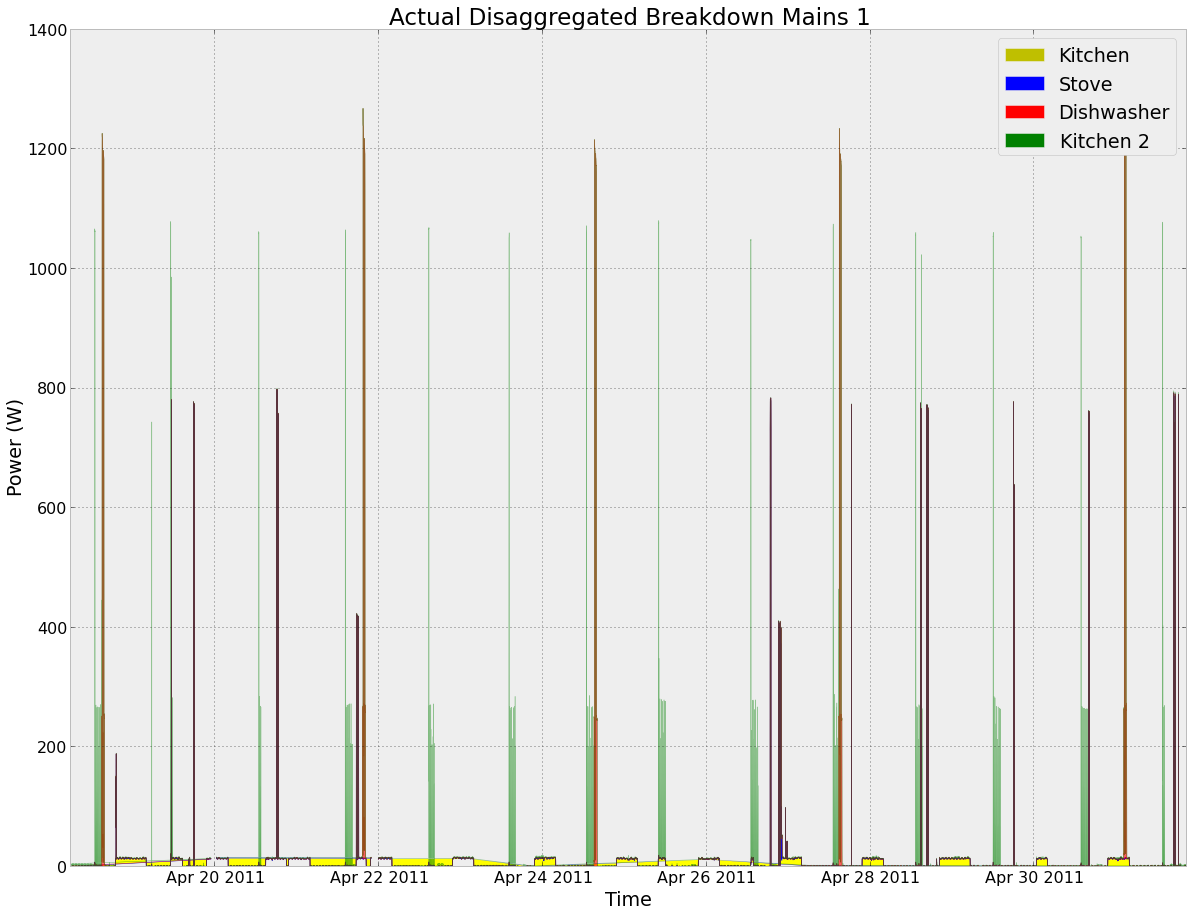
\includegraphics[width=0.7\textwidth]{REDD_House2_Analysis_files/REDD_House2_Analysis_fig_21.png}
\par
\end{center}
\end{codeoutput}
\end{codecell}
\subsection{State Space}
Finding different states for each appliance and the corresponding power
consumption using various clustering techniques. Firstly, we start with
stove. There are several reasons behind choosing a clustering algorithm,
some of them are mentioned at
http://scikit-learn.org/stable/modules/clustering.html

\begin{codecell}
\begin{codeinput}
\begin{lstlisting}
from sklearn.cluster import MiniBatchKMeans, KMeans
import time
plt.figsize(15,8)
\end{lstlisting}
\end{codeinput}
\end{codecell}
Filling missing data (currently NaN) with previous value (commonly known
as forward filling).

\textbf{CONFIRM: If this is the right thing to do}.

\begin{codecell}
\begin{codeinput}
\begin{lstlisting}
df_appliances_minute.fillna(method='pad',inplace=True)
times=df_appliances_minute.index.to_pydatetime()
raw_data={}
for key in df_appliances_minute:
    raw_data[key]=df_appliances_minute[key].values
    length=len(raw_data[key])
    raw_data[key]=raw_data[key].reshape(length,1)
\end{lstlisting}
\end{codeinput}
\end{codecell}
\begin{codecell}
\begin{codeinput}
\begin{lstlisting}
for key in df_appliances_minute:
    df_appliances_minute[key].to_csv(key+".arff",index_label=False,index=False)
\end{lstlisting}
\end{codeinput}
\end{codecell}
\begin{codecell}
\begin{codeinput}
\begin{lstlisting}
    batch_size=1000
def apply_kmeans(n_clusters, n_init,X,init=None):
    if init is None:
        k_means = KMeans(n_clusters=n_clusters, n_init=n_init)
    else:
        k_means=KMeans(init='k-means++',n_clusters=n_clusters, n_init=n_init)
    t0 = time.time()
    k_means.fit(X)
    t_batch = time.time() - t0
    k_means_labels = k_means.labels_
    k_means_cluster_centers = k_means.cluster_centers_
    k_means_labels_unique = np.unique(k_means_labels)
    k_means_inertia=k_means.inertia_
    mbk = MiniBatchKMeans(init='k-means++', n_clusters=n_clusters, batch_size=batch_size,
                      n_init=n_init, max_no_improvement=10, verbose=0)
    t0 = time.time()
    mbk.fit(X)
    t_mini_batch = time.time() - t0
    mbk_means_labels = mbk.labels_
    mbk_means_cluster_centers = mbk.cluster_centers_
    mbk_means_labels_unique = np.unique(mbk_means_labels)
    mbk_inertia=mbk.inertia_
    return [t_batch, t_mini_batch, k_means_labels, mbk_means_labels, k_means_cluster_centers, mbk_means_cluster_centers,\
    k_means_labels_unique,mbk_means_labels_unique, k_means_inertia, mbk_inertia] 
\end{lstlisting}
\end{codeinput}
\end{codecell}
\begin{codecell}
\begin{codeinput}
\begin{lstlisting}
def plot_cluster_assignments(X,k_means_labels, mbk_means_labels,k_means_cluster_centers,mbk_means_cluster_centers,n_clusters,appliance_name):
    colors = ['#4EACC5', '#FF9C34', '#4E9A06']
    markers=['o','*','.']
    x_temp=np.arange(len(X))
    plt.subplot(2,2,1)
    plt.rcParams["font.size"]=10
    print "\nKMeans Analysis\n"
    print "-"*80
    for k, col in zip(range(n_clusters), colors):
        my_members = k_means_labels == k
        cluster_center = k_means_cluster_centers[k]    
        plt.ylabel('Power (W)');
        plt.plot(x_temp[my_members],X[my_members, 0],markers[k],markersize=10,markerfacecolor=col) 
        plt.axhline(k_means_cluster_centers[k],linewidth=3,color=col)
        print "State %d Centroid= %0.4f, Fraction of datapoints= %0.4f" %(k,cluster_center,sum(my_members)*1.0/np.size(X))
        plt.title('KMeans Cluster Assignment for '+appliance_name+' for K='+str(n_clusters))
    plt.subplot(2,2,2)
    print "\nMini Batch KMeans Analysis\n"
    print "-"*80
    for k, col in zip(range(n_clusters), colors):
        my_members = mbk_means_labels == k
        cluster_center = mbk_means_cluster_centers[k]    
        plt.ylabel('Power (W)');
        plt.plot(x_temp[my_members],X[my_members, 0],markers[k],markersize=10,markerfacecolor=col) 
        plt.axhline(mbk_means_cluster_centers[k],linewidth=3,color=col)
        print "State %d Centroid= %0.4f, Fraction of datapoints= %0.4f" %(k,cluster_center,sum(my_members)*1.0/np.size(X))
        plt.title('Mini Batch KMeans Cluster Assignment for '+appliance_name+' for K='+str(n_clusters))
    print "-"*80
\end{lstlisting}
\end{codeinput}
\end{codecell}
\begin{codecell}
\begin{codeinput}
\begin{lstlisting}
[t_batch, t_mini_batch, k_means_labels, mbk_means_labels, k_means_cluster_centers, mbk_means_cluster_centers,
    k_means_labels_unique,mbk_means_labels_unique, k_means_inertia, mbk_inertia]=apply_kmeans(2,10,raw_data["stove"],"kmeans++")
plot_cluster_assignments(raw_data["stove"],k_means_labels, mbk_means_labels, k_means_cluster_centers, mbk_means_cluster_centers\
,2,"Stove")
print "Time taken for Kmeans clustering    :     \n",t_batch
print "Inertia of KMeans cluster assignment:     \n",k_means_inertia
print "Time taken for Mini Batch Kmeans clustering    :     \n",t_mini_batch
print "Inertia of Mini Batch KMeans cluster assignment:     \n",mbk_inertia
\end{lstlisting}
\end{codeinput}
\begin{codeoutput}
\begin{verbatim}
KMeans Analysis

--------------------------------------------------------------------------------
State 0 Centroid= 0.6480, Fraction of datapoints= 0.9978
State 1 Centroid= 374.0394, Fraction of datapoints= 0.0022

Mini Batch KMeans Analysis

--------------------------------------------------------------------------------
State 0 Centroid= 0.6800, Fraction of datapoints= 0.9978
State 1 Centroid= 369.7725, Fraction of datapoints= 0.0022
--------------------------------------------------------------------------------
Time taken for Kmeans clustering    :
\end{verbatim}
\begin{verbatim}
0.054370880127
Inertia of KMeans cluster assignment:     
361045.705434
Time taken for Mini Batch Kmeans clustering    :     
0.0232241153717
Inertia of Mini Batch KMeans cluster assignment:     
361848.586124
\end{verbatim}
\begin{center}
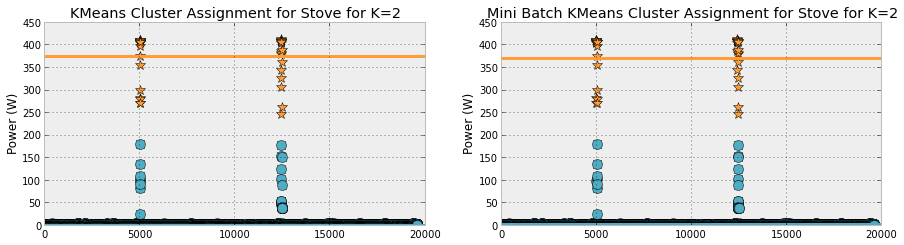
\includegraphics[width=0.7\textwidth]{REDD_House2_Analysis_files/REDD_House2_Analysis_fig_22.png}
\par
\end{center}
\end{codeoutput}
\end{codecell}
\begin{codecell}
\begin{codeinput}
\begin{lstlisting}
[t_batch, t_mini_batch, k_means_labels, mbk_means_labels, k_means_cluster_centers, mbk_means_cluster_centers,
    k_means_labels_unique,mbk_means_labels_unique, k_means_inertia, mbk_inertia]=apply_kmeans(2,10,raw_data["kitchen"],"kmeans++")
plot_cluster_assignments(raw_data["kitchen"],k_means_labels, mbk_means_labels, k_means_cluster_centers, mbk_means_cluster_centers\
,2,"Kitchen")
print "Time taken for Kmeans clustering    :     \n",t_batch
print "Inertia of KMeans cluster assignment:     \n",k_means_inertia
print "Time taken for Mini Batch Kmeans clustering    :     \n",t_mini_batch
print "Inertia of Mini Batch KMeans cluster assignment:     \n",mbk_inertia
\end{lstlisting}
\end{codeinput}
\begin{codeoutput}
\begin{verbatim}
KMeans Analysis

--------------------------------------------------------------------------------
State 0 Centroid= 4.5853, Fraction of datapoints= 0.9976
State 1 Centroid= 671.6462, Fraction of datapoints= 0.0024

Mini Batch KMeans Analysis

--------------------------------------------------------------------------------
State 0 Centroid= 4.4589, Fraction of datapoints= 0.9976
State 1 Centroid= 669.6980, Fraction of datapoints= 0.0024
--------------------------------------------------------------------------------
Time taken for Kmeans clustering    :
\end{verbatim}
\begin{verbatim}
0.0747680664062
Inertia of KMeans cluster assignment:     
2529066.47693
Time taken for Mini Batch Kmeans clustering    :     
0.0225470066071
Inertia of Mini Batch KMeans cluster assignment:     
2529561.55892
\end{verbatim}
\begin{center}
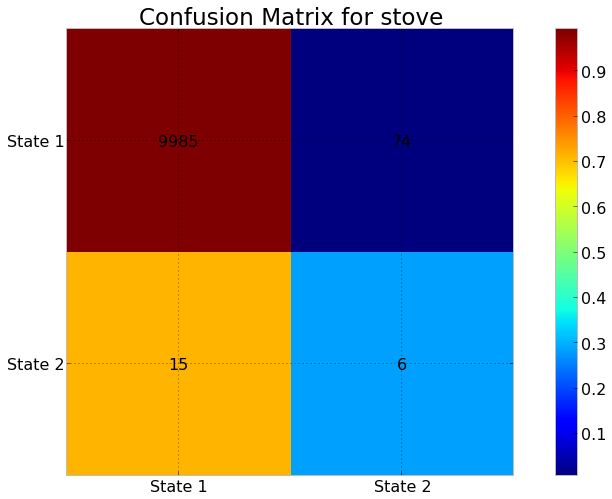
\includegraphics[width=0.7\textwidth]{REDD_House2_Analysis_files/REDD_House2_Analysis_fig_23.png}
\par
\end{center}
\end{codeoutput}
\end{codecell}
\begin{codecell}
\begin{codeinput}
\begin{lstlisting}
[t_batch, t_mini_batch, k_means_labels, mbk_means_labels, k_means_cluster_centers, mbk_means_cluster_centers,
    k_means_labels_unique,mbk_means_labels_unique, k_means_inertia, mbk_inertia]=apply_kmeans(3,10,raw_data["kitchen_2"],"kmeans++")
plot_cluster_assignments(raw_data["kitchen_2"],k_means_labels, mbk_means_labels, k_means_cluster_centers, mbk_means_cluster_centers\
,3,"Kitchen 2")
print "Time taken for Kmeans clustering    :     \n",t_batch
print "Inertia of KMeans cluster assignment:     \n",k_means_inertia
print "Time taken for Mini Batch Kmeans clustering    :     \n",t_mini_batch
print "Inertia of Mini Batch KMeans cluster assignment:     \n",mbk_inertia
\end{lstlisting}
\end{codeinput}
\begin{codeoutput}
\begin{verbatim}
KMeans Analysis

--------------------------------------------------------------------------------
State 0 Centroid= 1.4546, Fraction of datapoints= 0.9729
State 1 Centroid= 1035.4956, Fraction of datapoints= 0.0042
State 2 Centroid= 205.6050, Fraction of datapoints= 0.0229

Mini Batch KMeans Analysis

--------------------------------------------------------------------------------
State 0 Centroid= 1.3577, Fraction of datapoints= 0.9729
State 1 Centroid= 1043.7727, Fraction of datapoints= 0.0042
State 2 Centroid= 204.7535, Fraction of datapoints= 0.0229
--------------------------------------------------------------------------------
Time taken for Kmeans clustering    :
\end{verbatim}
\begin{verbatim}
0.0749089717865
Inertia of KMeans cluster assignment:     
2805123.96163
Time taken for Mini Batch Kmeans clustering    :     
0.0284309387207
Inertia of Mini Batch KMeans cluster assignment:     
2811246.58659
\end{verbatim}
\begin{center}
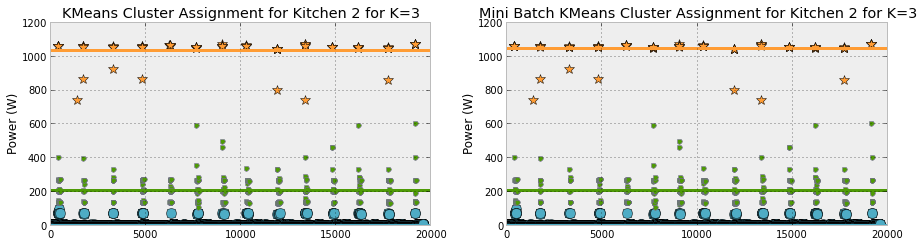
\includegraphics[width=0.7\textwidth]{REDD_House2_Analysis_files/REDD_House2_Analysis_fig_24.png}
\par
\end{center}
\end{codeoutput}
\end{codecell}
\begin{codecell}
\begin{codeinput}
\begin{lstlisting}
[t_batch, t_mini_batch, k_means_labels, mbk_means_labels, k_means_cluster_centers, mbk_means_cluster_centers,
    k_means_labels_unique,mbk_means_labels_unique, k_means_inertia, mbk_inertia]=apply_kmeans(3,10,raw_data["dishwasher"],"kmeans++")
plot_cluster_assignments(raw_data["dishwasher"],k_means_labels, mbk_means_labels, k_means_cluster_centers, mbk_means_cluster_centers\
,3,"Dishwasher")
print "Time taken for Kmeans clustering    :     \n",t_batch
print "Inertia of KMeans cluster assignment:     \n",k_means_inertia
print "Time taken for Mini Batch Kmeans clustering    :     \n",t_mini_batch
print "Inertia of Mini Batch KMeans cluster assignment:     \n",mbk_inertia
\end{lstlisting}
\end{codeinput}
\begin{codeoutput}
\begin{verbatim}
KMeans Analysis

--------------------------------------------------------------------------------
State 0 Centroid= 0.1364, Fraction of datapoints= 0.9874
State 1 Centroid= 1186.5108, Fraction of datapoints= 0.0063
State 2 Centroid= 249.6954, Fraction of datapoints= 0.0063

Mini Batch KMeans Analysis

--------------------------------------------------------------------------------
State 0 Centroid= 0.1670, Fraction of datapoints= 0.9874
State 1 Centroid= 1185.8841, Fraction of datapoints= 0.0063
State 2 Centroid= 259.9662, Fraction of datapoints= 0.0063
\end{verbatim}
\begin{verbatim}
--------------------------------------------------------------------------------
Time taken for Kmeans clustering    :     
0.0705690383911
Inertia of KMeans cluster assignment:     
1339180.63283
Time taken for Mini Batch Kmeans clustering    :     
0.0283811092377
Inertia of Mini Batch KMeans cluster assignment:     
1352327.68731
\end{verbatim}
\begin{center}
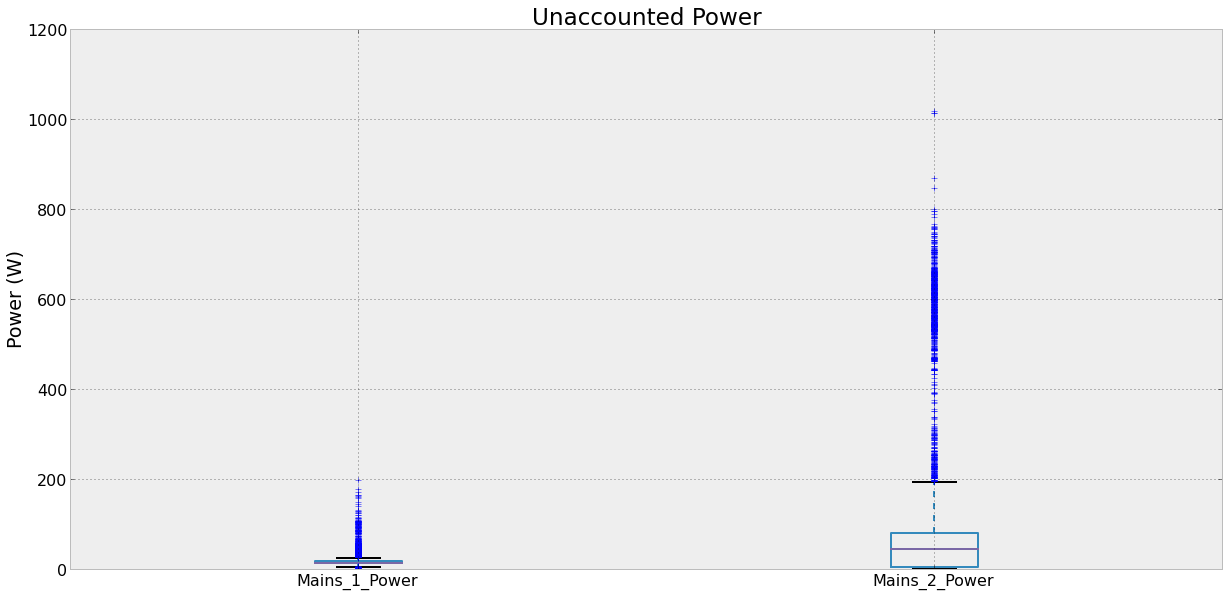
\includegraphics[width=0.7\textwidth]{REDD_House2_Analysis_files/REDD_House2_Analysis_fig_25.png}
\par
\end{center}
\end{codeoutput}
\end{codecell}
\begin{codecell}
\begin{codeinput}
\begin{lstlisting}
[t_batch, t_mini_batch, k_means_labels, mbk_means_labels, k_means_cluster_centers, mbk_means_cluster_centers,
    k_means_labels_unique,mbk_means_labels_unique, k_means_inertia, mbk_inertia]=apply_kmeans(3,10,raw_data["refrigerator"],"kmeans++")
plot_cluster_assignments(raw_data["refrigerator"],k_means_labels, mbk_means_labels, k_means_cluster_centers, mbk_means_cluster_centers\
,3,"Refrigerator")
print "Time taken for Kmeans clustering    :     \n",t_batch
print "Inertia of KMeans cluster assignment:     \n",k_means_inertia
print "Time taken for Mini Batch Kmeans clustering    :     \n",t_mini_batch
print "Inertia of Mini Batch KMeans cluster assignment:     \n",mbk_inertia
\end{lstlisting}
\end{codeinput}
\begin{codeoutput}
\begin{verbatim}
KMeans Analysis

--------------------------------------------------------------------------------
State 0 Centroid= 7.4725, Fraction of datapoints= 0.5538
State 1 Centroid= 162.1867, Fraction of datapoints= 0.4327
State 2 Centroid= 394.8063, Fraction of datapoints= 0.0136

Mini Batch KMeans Analysis

--------------------------------------------------------------------------------
State 0 Centroid= 7.5489, Fraction of datapoints= 0.5538
State 1 Centroid= 162.2095, Fraction of datapoints= 0.4327
State 2 Centroid= 395.7196, Fraction of datapoints= 0.0136
--------------------------------------------------------------------------------
Time taken for Kmeans clustering    :
\end{verbatim}
\begin{verbatim}
0.0944950580597
Inertia of KMeans cluster assignment:     
2597652.90778
Time taken for Mini Batch Kmeans clustering    :     
0.048819065094
Inertia of Mini Batch KMeans cluster assignment:     
2597942.56915
\end{verbatim}
\begin{center}
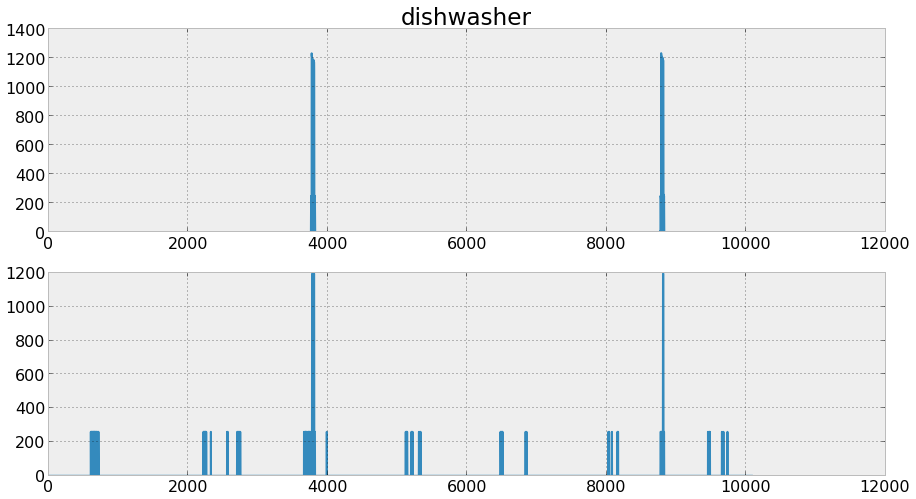
\includegraphics[width=0.7\textwidth]{REDD_House2_Analysis_files/REDD_House2_Analysis_fig_26.png}
\par
\end{center}
\end{codeoutput}
\end{codecell}
\begin{codecell}
\begin{codeinput}
\begin{lstlisting}
[t_batch, t_mini_batch, k_means_labels, mbk_means_labels, k_means_cluster_centers, mbk_means_cluster_centers,
    k_means_labels_unique,mbk_means_labels_unique, k_means_inertia, mbk_inertia]=apply_kmeans(3,10,raw_data["microwave"],"kmeans++")
plot_cluster_assignments(raw_data["microwave"],k_means_labels, mbk_means_labels, k_means_cluster_centers, mbk_means_cluster_centers\
,3,"Microwave")
print "Time taken for Kmeans clustering    :     \n",t_batch
print "Inertia of KMeans cluster assignment:     \n",k_means_inertia
print "Time taken for Mini Batch Kmeans clustering    :     \n",t_mini_batch
print "Inertia of Mini Batch KMeans cluster assignment:     \n",mbk_inertia
\end{lstlisting}
\end{codeinput}
\begin{codeoutput}
\begin{verbatim}
KMeans Analysis

--------------------------------------------------------------------------------
State 0 Centroid= 8.6130, Fraction of datapoints= 0.9952
State 1 Centroid= 1677.3997, Fraction of datapoints= 0.0020
State 2 Centroid= 852.9569, Fraction of datapoints= 0.0029

Mini Batch KMeans Analysis

--------------------------------------------------------------------------------
State 0 Centroid= 8.4798, Fraction of datapoints= 0.9951
State 1 Centroid= 1601.1895, Fraction of datapoints= 0.0023
State 2 Centroid= 740.9955, Fraction of datapoints= 0.0026
\end{verbatim}
\begin{verbatim}
--------------------------------------------------------------------------------
Time taken for Kmeans clustering    :     
0.187880992889
Inertia of KMeans cluster assignment:     
8371412.23135
Time taken for Mini Batch Kmeans clustering    :     
0.0284819602966
Inertia of Mini Batch KMeans cluster assignment:     
8642849.35369
\end{verbatim}
\begin{center}
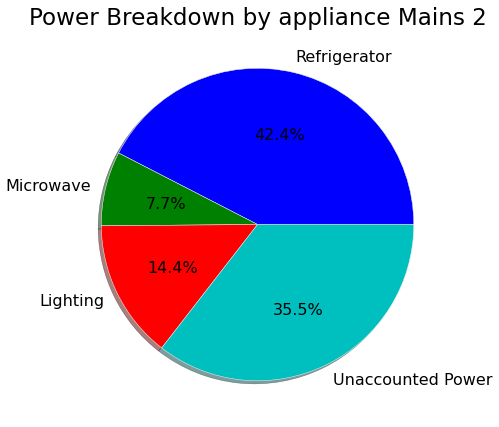
\includegraphics[width=0.7\textwidth]{REDD_House2_Analysis_files/REDD_House2_Analysis_fig_27.png}
\par
\end{center}
\end{codeoutput}
\end{codecell}
\begin{codecell}
\begin{codeinput}
\begin{lstlisting}
[t_batch, t_mini_batch, k_means_labels, mbk_means_labels, k_means_cluster_centers, mbk_means_cluster_centers,
    k_means_labels_unique,mbk_means_labels_unique, k_means_inertia, mbk_inertia]=apply_kmeans(3,10,raw_data["light"],"kmeans++")
plot_cluster_assignments(raw_data["light"],k_means_labels, mbk_means_labels, k_means_cluster_centers, mbk_means_cluster_centers\
,3,"Light")
print "Time taken for Kmeans clustering    :     \n",t_batch
print "Inertia of KMeans cluster assignment:     \n",k_means_inertia
print "Time taken for Mini Batch Kmeans clustering    :     \n",t_mini_batch
print "Inertia of Mini Batch KMeans cluster assignment:     \n",mbk_inertia
\end{lstlisting}
\end{codeinput}
\begin{codeoutput}
\begin{verbatim}
KMeans Analysis

--------------------------------------------------------------------------------
State 0 Centroid= 9.5566, Fraction of datapoints= 0.8668
State 1 Centroid= 155.5247, Fraction of datapoints= 0.1033
State 2 Centroid= 96.5077, Fraction of datapoints= 0.0299

Mini Batch KMeans Analysis

--------------------------------------------------------------------------------
State 0 Centroid= 9.5453, Fraction of datapoints= 0.8668
State 1 Centroid= 155.5140, Fraction of datapoints= 0.1033
State 2 Centroid= 96.0181, Fraction of datapoints= 0.0299
--------------------------------------------------------------------------------
Time taken for Kmeans clustering    :
\end{verbatim}
\begin{verbatim}
0.0899589061737
Inertia of KMeans cluster assignment:     
508702.879442
Time taken for Mini Batch Kmeans clustering    :     
0.0430018901825
Inertia of Mini Batch KMeans cluster assignment:     
508845.969858
\end{verbatim}
\begin{center}
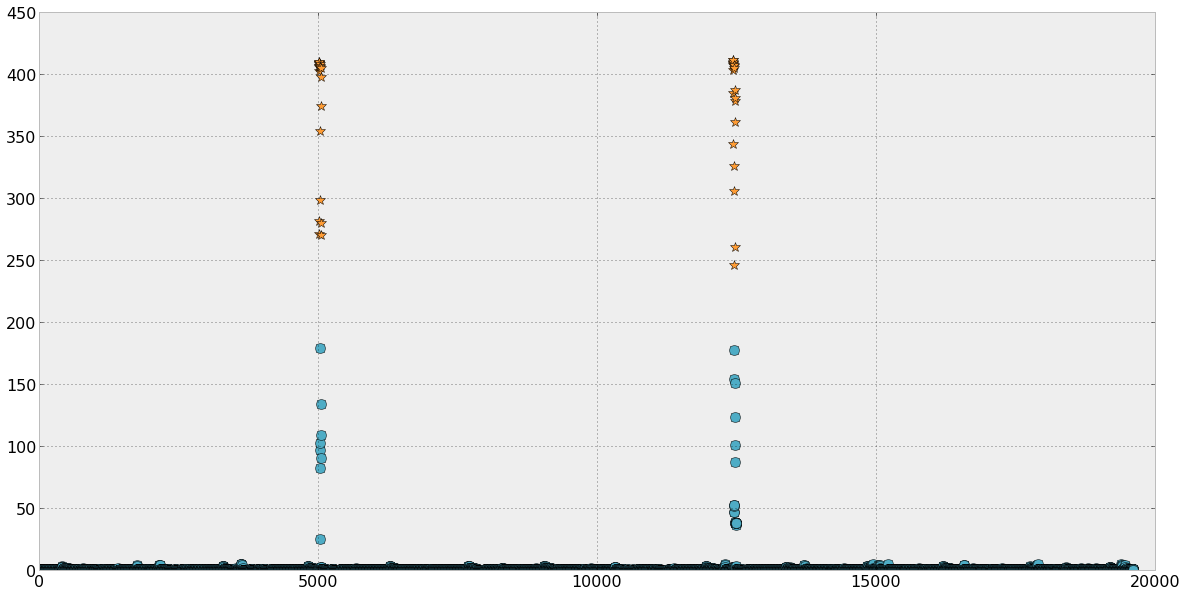
\includegraphics[width=0.7\textwidth]{REDD_House2_Analysis_files/REDD_House2_Analysis_fig_28.png}
\par
\end{center}
\end{codeoutput}
\end{codecell}
\begin{codecell}
\begin{codeinput}
\begin{lstlisting}
from scipy.spatial import distance
from sklearn.cluster import DBSCAN
\end{lstlisting}
\end{codeinput}
\end{codecell}
We also tried different a different distance metric like Manhattan
distance in Weka, which led to absurd results and mostly single class
being predicted.

\textbf{Tried to do DBScan in scikit learn, but it took too much memory
and time and hung the system}

DBSCan in Weka took about 30s and resulted in all attributed being
classified in one cluster. This may be due to the nature of the data,
which is 1 class majority. This again may be something to look into.
While dealing with such data we are mostly going to encounter datasets
which are heavy in a single class. \textbf{This is again something,
which i don't think has been talked in NILM literature before.}

SOM based clustering took about 30s per appliance, but yielded much
better results, which are shown below. EM took about 42 seconds and the
results are not too impressive.

\begin{codecell}
\begin{codeinput}
\begin{lstlisting}
from IPython.core.display import Image 
Image(filename='som_ref.png') 
\end{lstlisting}
\end{codeinput}
\begin{codeoutput}
\begin{verbatim}
<IPython.core.display.Image at 0x82ac4d0>
\end{verbatim}
\end{codeoutput}
\end{codecell}
\begin{codecell}
\begin{codeinput}
\begin{lstlisting}
Image(filename='som_stove.png') 
\end{lstlisting}
\end{codeinput}
\begin{codeoutput}
\begin{verbatim}
<IPython.core.display.Image at 0x82ac810>
\end{verbatim}
\end{codeoutput}
\end{codecell}
Thus, we obtain the following states from cluster analysis (results are
from KMeans). \textbf{In the above results we also saw that most of the
appliances are mostly in their off states most of the time. This is an
important aspect and must be exploited.}

\begin{codecell}
\begin{codeinput}
\begin{lstlisting}
kitchen=[5,672]
lighting=[9,96,155]
stove=[0,374]
micro=[8,852,1677]
kitchen_2=[1,206,1035]
ref=[7,162,394]
dish=[0,250,1186]
\end{lstlisting}
\end{codeinput}
\end{codecell}
For mains 1, we now draw the state space, which consists of all possible
combinations of appliances in their different states. We also show the
correpsonding histogram which tells how close the different states are.
The closer the states, the more difficult the disaggregation becomes.

\begin{codecell}
\begin{codeinput}
\begin{lstlisting}
states_combination=list(itertools.product(kitchen,stove,kitchen_2,dish))
\end{lstlisting}
\end{codeinput}
\end{codecell}
\begin{codecell}
\begin{codeinput}
\begin{lstlisting}
print "The possible different state combinations are\n Kitchen, Stove, Kitchen 2, Dishwasher\n",states_combination
\end{lstlisting}
\end{codeinput}
\begin{codeoutput}
\begin{verbatim}
The possible different state combinations are
 Kitchen, Stove, Kitchen 2, Dishwasher
[(5, 0, 1, 0), (5, 0, 1, 250), (5, 0, 1, 1186), (5, 0, 206, 0), (5, 0, 206, 250), (5, 0, 206, 1186), (5, 0, 1035, 0), (5, 0, 1035, 250), (5, 0, 1035, 1186), (5, 374, 1, 0), (5, 374, 1, 250), (5, 374, 1, 1186), (5, 374, 206, 0), (5, 374, 206, 250), (5, 374, 206, 1186), (5, 374, 1035, 0), (5, 374, 1035, 250), (5, 374, 1035, 1186), (672, 0, 1, 0), (672, 0, 1, 250), (672, 0, 1, 1186), (672, 0, 206, 0), (672, 0, 206, 250), (672, 0, 206, 1186), (672, 0, 1035, 0), (672, 0, 1035, 250), (672, 0, 1035, 1186), (672, 374, 1, 0), (672, 374, 1, 250), (672, 374, 1, 1186), (672, 374, 206, 0), (672, 374, 206, 250), (672, 374, 206, 1186), (672, 374, 1035, 0), (672, 374, 1035, 250), (672, 374, 1035, 1186)]
\end{verbatim}
\end{codeoutput}
\end{codecell}
\begin{codecell}
\begin{codeinput}
\begin{lstlisting}
sum_combination=np.array(np.zeros(len(states_combination)))
for i in range(0,len(states_combination)):
    sum_combination[i]=sum(states_combination[i])
from copy import deepcopy
b=deepcopy(sum_combination)
b.sort()
grid(True)
title('Sorted possible sums of all appliances');
plt.xlabel('Combinations');
plt.ylabel('Power (W)');
plt.plot(b,'go-',markersize=8,linewidth=3);
\end{lstlisting}
\end{codeinput}
\begin{codeoutput}
\begin{center}
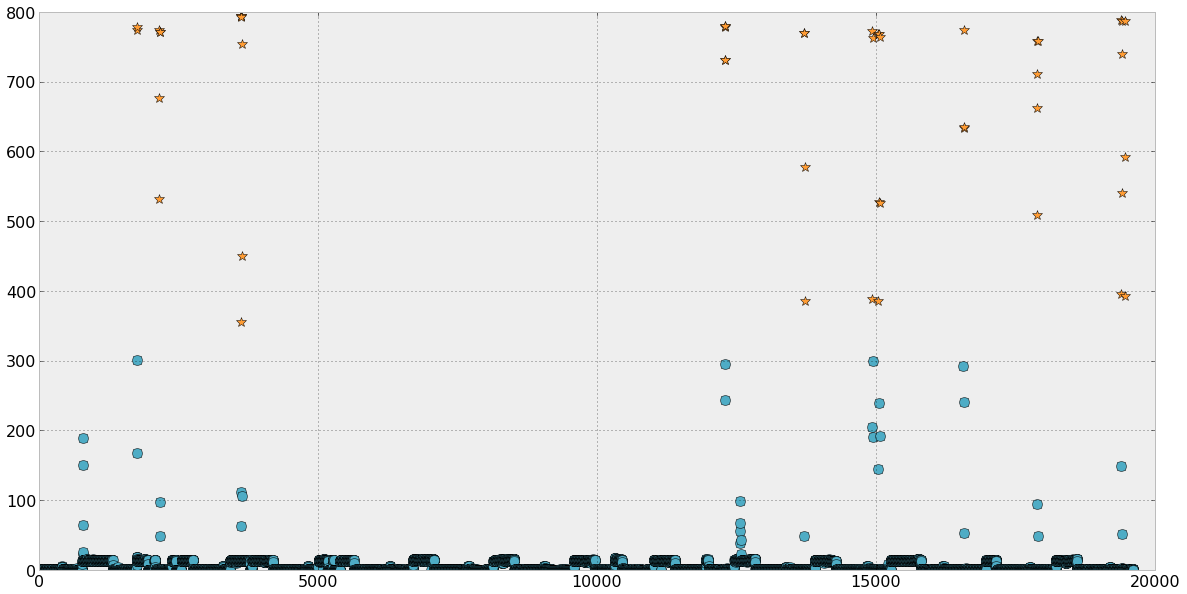
\includegraphics[width=0.7\textwidth]{REDD_House2_Analysis_files/REDD_House2_Analysis_fig_29.png}
\par
\end{center}
\end{codeoutput}
\end{codecell}
\begin{codecell}
\begin{codeinput}
\begin{lstlisting}
plt.title('Histogram showing relative frequencies of different state combinations');
plt.hist(b,20);
\end{lstlisting}
\end{codeinput}
\begin{codeoutput}
\begin{center}
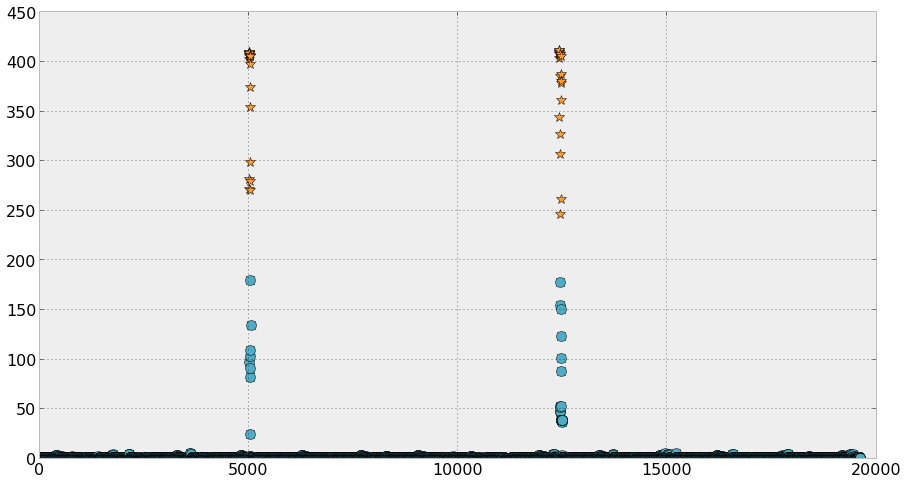
\includegraphics[width=0.7\textwidth]{REDD_House2_Analysis_files/REDD_House2_Analysis_fig_30.png}
\par
\end{center}
\end{codeoutput}
\end{codecell}
Now we basically need to iterate over all our sample and see which of
the possible state assignment matches closest to the overall power
consumption. We thus create a function to do the same.

\begin{codecell}
\begin{codeinput}
\begin{lstlisting}
def find_nearest(array,value):
    idx = (np.abs(array-value)).argmin()
    diff=array[idx]-value
    return [idx,-diff]
\end{lstlisting}
\end{codeinput}
\end{codecell}
We thus apply this technique to find the residual power left from the
closest state assignment.

\begin{codecell}
\begin{codeinput}
\begin{lstlisting}
residual_power_mains_1=np.zeros(len(filtered_downsampled_mains_1))
states_idx=np.zeros(len(filtered_downsampled_mains_1))                               
for i in range(len(filtered_downsampled_mains_1)):
    [states_idx[i],residual_power_mains_1[i]]=find_nearest(sum_combination,filtered_downsampled_mains_1[i])

\end{lstlisting}
\end{codeinput}
\end{codecell}
\begin{codecell}
\begin{codeinput}
\begin{lstlisting}
title('Residual Power Mains 1');
xlabel('Time');
ylabel('Power (W)');
plot(residual_power_mains_1);
\end{lstlisting}
\end{codeinput}
\end{codecell}
However we can also impose another conditon that the sum of powers of
all the appliances is strictly less than the aggregate power observed.
Thus, we can create a function for that as follows.

\begin{codecell}
\begin{codeinput}
\begin{lstlisting}
def find_nearest_positive(array,value):    
    idx_temp = np.where(array-value<=0.0)[0]
    temp_arr=array[idx_temp]
    try:
        idx_in_new=np.abs(temp_arr-value).argmin()
        idx=np.where(array==temp_arr[idx_in_new])[0][0]

        diff=array[idx]-value
    except:
        idx=0
        diff=0
    return [idx,-diff]
\end{lstlisting}
\end{codeinput}
\end{codecell}
\begin{codecell}
\begin{codeinput}
\begin{lstlisting}
residual_power_mains_1_positive=np.zeros(len(filtered_downsampled_mains_1))
states_idx_positive=np.zeros(len(filtered_downsampled_mains_1))
residual_power_mains_2=np.zeros(len(filtered_downsampled_mains_2))
states_idx_2=np.zeros(len(filtered_downsampled_mains_1))
for i in range(len(filtered_downsampled_mains_1)):
    [states_idx_positive[i],residual_power_mains_1_positive[i]]=find_nearest_positive(sum_combination,filtered_downsampled_mains_1[i])

\end{lstlisting}
\end{codeinput}
\end{codecell}
\begin{codecell}
\begin{codeinput}
\begin{lstlisting}
title('Residual Power Mains 1 considering sum of appliance powers < Aggregate Power');
xlabel('Time');
ylabel('Power (W)');
grid(True);
plot(residual_power_mains_1_positive);

\end{lstlisting}
\end{codeinput}
\end{codecell}
After having applied Total Load Model, we need to assign different
states to different appliances.

\begin{codecell}
\begin{codeinput}
\begin{lstlisting}
length_sequence=len(filtered_downsampled_mains_1)
co_kitchen_states=np.zeros(length_sequence,dtype=np.int)
co_kitchen_power=np.zeros(length_sequence)
co_stove_states=np.zeros(length_sequence,dtype=np.int)
co_stove_power=np.zeros(length_sequence)
co_kitchen_2_states=np.zeros(length_sequence,dtype=np.int)
co_kitchen_2_power=np.zeros(length_sequence)
co_dish_states=np.zeros(length_sequence,dtype=np.int)
co_dish_power=np.zeros(length_sequence)

\end{lstlisting}
\end{codeinput}
\end{codecell}
\begin{codecell}
\begin{codeinput}
\begin{lstlisting}
for i in range(length_sequence):
    if int(states_idx[i])/18==0:
        co_kitchen_states[i]=0
        
    else:
        co_kitchen_states[i]=1
    co_kitchen_power[i]=kitchen[co_kitchen_states[i]]   
    
    temp=int(states_idx[i])/9
    if temp%2==0:
        co_stove_states[i]=0
    else:
        co_stove_states[i]=1
    co_stove_power[i]=stove[co_stove_states[i]]
    
    temp=int(states_idx[i])/3
    if temp%3==0:
        co_kitchen_2_states[i]=0
    elif temp%3==1:
        co_kitchen_2_states[i]=1
    else:
        co_kitchen_2_states[i]=2
    co_kitchen_2_power[i]=kitchen_2[co_kitchen_2_states[i]]
    
    temp=int(states_idx[i])%3
    if temp==0:
        co_dish_states[i]=0
    elif temp==1:
        co_dish_states[i]=1
    else:
        co_dish_states[i]=2
    co_dish_power[i]=dish[co_dish_states[i]]       
\end{lstlisting}
\end{codeinput}
\end{codecell}
Now we compare the produced output with Ground truth.

\begin{codecell}
\begin{codeinput}
\begin{lstlisting}
subplot(2,1,1);

plt.title('Actual Dishwasher Consumption');
plt.xlabel('Time');
plt.ylabel('Power (W)');
subplots_adjust(hspace=.5)
plt.plot(downsampled_timestamp_appliance_date,downsampled_dishwasher);
subplot(2,1,2);
plt.xlabel('Time');
plt.ylabel('Power (W)');
plt.title('Observed Dishwasher Consumption');
plt.plot(downsampled_timestamp_appliance_date,co_dish_power);          
\end{lstlisting}
\end{codeinput}
\end{codecell}
\begin{codecell}
\begin{codeinput}
\begin{lstlisting}
plt.subplot(2,1,1)
plt.title('Actual Kitchen 1 Consumption');
plt.xlabel('Time');
plt.ylabel('Power (W)');
subplots_adjust(hspace=.5);
plt.plot(downsampled_timestamp_appliance_date,downsampled_kitchen)
plt.subplot(2,1,2)
plt.xlabel('Time');
plt.ylabel('Power (W)');
plt.title('Observed Kitchen 1 Consumption')
plt.ylim((0,800))
plt.plot(downsampled_timestamp_appliance_date,co_kitchen_power);
\end{lstlisting}
\end{codeinput}
\end{codecell}
\begin{codecell}
\begin{codeinput}
\begin{lstlisting}
plt.subplot(2,1,1)
plt.title('Actual Kitchen 2 Consumption')
plt.xlabel('Time');
plt.ylabel('Power (W)');
subplots_adjust(hspace=.5);
plt.plot(downsampled_timestamp_appliance_date,downsampled_kitchen_2)
plt.subplot(2,1,2)
plt.xlabel('Time');
plt.ylabel('Power (W)');
plt.title('Observed Kitchen 2 Consumption')
plt.plot(downsampled_timestamp_appliance_date,co_kitchen_2_power);
\end{lstlisting}
\end{codeinput}
\end{codecell}
\begin{codecell}
\begin{codeinput}
\begin{lstlisting}
plt.subplot(2,1,1)
plt.title('Actual Stove Consumption')
plt.xlabel('Time');
plt.ylabel('Power (W)');
subplots_adjust(hspace=.5)
plt.plot(downsampled_timestamp_appliance_date,downsampled_stove)
plt.subplot(2,1,2)
plt.xlabel('Time');
plt.ylabel('Power (W)');
plt.title('Predicted Stove Consumption')
plt.plot(downsampled_timestamp_appliance_date,co_stove_power);
\end{lstlisting}
\end{codeinput}
\end{codecell}
Calculation of Residual Power and Standard Deviation

\begin{codecell}
\begin{codeinput}
\begin{lstlisting}
residual_power_total=sum(np.abs(residual_power_mains_1))
print "Residual Power is: ",residual_power_total," W"
standard_deviation=np.std(residual_power_mains_1)
print "Standard Deviation is ",standard_deviation
\end{lstlisting}
\end{codeinput}
\end{codecell}
Reading original labels of different states for different appliances

\begin{codecell}
\begin{codeinput}
\begin{lstlisting}
dummy,labels_stove=np.loadtxt('clustered_stove')
dummy,labels_kitchen=np.loadtxt('clustered_kitchen')
dummy,labels_kitchen_2=np.loadtxt('clustered_kitchen_2')
dummy,labels_dish=np.loadtxt('clustered_dishwasher')
dummy,labels_ref=np.loadtxt('clustered_refrigerator')
dummy,labels_micro=np.loadtxt('clustered_microwave')
dummy,labels_lighting=np.loadtxt('clustered_lighting')
\end{lstlisting}
\end{codeinput}
\end{codecell}
\begin{codecell}
\begin{codeinput}
\begin{lstlisting}
labels_stove=labels_stove.astype(np.int)
labels_kitchen=labels_kitchen.astype(np.int)
labels_kitchen_2=labels_kitchen_2.astype(np.int)
labels_dish=labels_dish.astype(np.int)
labels_ref=labels_ref.astype(np.int)
labels_micro=labels_micro.astype(np.int)
labels_lighting=labels_lighting.astype(np.int)
\end{lstlisting}
\end{codeinput}
\end{codecell}
Next, we define a function to plot the confusion matrix.

\begin{codecell}
\begin{codeinput}
\begin{lstlisting}
def print_confusion_matrix(appliance,num_states,true_label,observed_label):
    correct_predicted=0
    conf_arr=[]
    for i in range(num_states):
        counts=[]
        for j in range(num_states):        
            idx=np.where(true_label==i)[0]
            counts.append(len(np.where(observed_label[idx]==j)[0]))
        correct_predicted+=counts[i]
        conf_arr.append(counts)
    
    norm_conf = []
    for i in conf_arr:
        a = 0
        tmp_arr = []
        a = sum(i, 0)
        for j in i:
            tmp_arr.append(float(j)/float(a))
        norm_conf.append(tmp_arr)

    fig = plt.figure()
    plt.clf()
    ax = fig.add_subplot(111)
    ax.set_aspect(1)
    res = ax.imshow(np.array(norm_conf), cmap=plt.cm.jet, 
                interpolation='nearest')

    width = len(conf_arr)
    height = len(conf_arr[0])

    for x in xrange(width):
        for y in xrange(height):
            ax.annotate(str(conf_arr[x][y]), xy=(y, x), 
                    horizontalalignment='center',
                    verticalalignment='center')

    cb = fig.colorbar(res)
    alphabet = ['State 1','State 2','State 3']
    plt.title('Confusion Matrix for '+appliance)
    plt.xticks(range(width), alphabet[:width])
    plt.yticks(range(height), alphabet[:height])
    plt.show()
    return correct_predicted*1.0/len(true_label)
    
        
\end{lstlisting}
\end{codeinput}
\end{codecell}
Plotting the confusion matices for different appliances mains 1

\begin{codecell}
\begin{codeinput}
\begin{lstlisting}
stove_accuracy=print_confusion_matrix("stove",len(stove),labels_stove,co_stove_states)
kitchen_accuracy=print_confusion_matrix("kitchen",len(kitchen),labels_kitchen,co_kitchen_states)
kitchen_2_accuracy=print_confusion_matrix("kitchen_2",len(kitchen_2),labels_kitchen_2,co_kitchen_2_states)
dishwasher_accuracy=print_confusion_matrix("dishwasher",len(dish),labels_dish,co_dish_states)
\end{lstlisting}
\end{codeinput}
\end{codecell}
We now repeat the same procedure when we take the assumption that the
sum of powers of different appliances must be less than or equal to the
aggregate power.

\begin{codecell}
\begin{codeinput}
\begin{lstlisting}
co_positive_kitchen_states=np.zeros(length_sequence,dtype=np.int)
co_positive_kitchen_power=np.zeros(length_sequence)
co_positive_stove_states=np.zeros(length_sequence,dtype=np.int)
co_positive_stove_power=np.zeros(length_sequence)
co_positive_kitchen_2_states=np.zeros(length_sequence,dtype=np.int)
co_positive_kitchen_2_power=np.zeros(length_sequence)
co_positive_dish_states=np.zeros(length_sequence,dtype=np.int)
co_positive_dish_power=np.zeros(length_sequence)
\end{lstlisting}
\end{codeinput}
\end{codecell}
\begin{codecell}
\begin{codeinput}
\begin{lstlisting}
for i in range(length_sequence):
    if int(states_idx_positive[i])/18==0:
        co_positive_kitchen_states[i]=0
        
    else:
        co_positive_kitchen_states[i]=1
    co_positive_kitchen_power[i]=kitchen[co_positive_kitchen_states[i]]   
    
    temp=int(states_idx_positive[i])/9
    if temp%2==0:
        co_positive_stove_states[i]=0
    else:
        co_positive_stove_states[i]=1
    co_positive_stove_power[i]=stove[co_positive_stove_states[i]]
    
    temp=int(states_idx_positive[i])/3
    if temp%3==0:
        co_positive_kitchen_2_states[i]=0
    elif temp%3==1:
        co_positive_kitchen_2_states[i]=1
    else:
        co_positive_kitchen_2_states[i]=2
    co_positive_kitchen_2_power[i]=kitchen_2[co_positive_kitchen_2_states[i]]
    
    temp=int(states_idx_positive[i])%3
    if temp==0:
        co_positive_dish_states[i]=0
    elif temp==1:
        co_positive_dish_states[i]=1
    else:
        co_positive_dish_states[i]=2
    co_positive_dish_power[i]=dish[co_positive_dish_states[i]]
\end{lstlisting}
\end{codeinput}
\end{codecell}
\begin{codecell}
\begin{codeinput}
\begin{lstlisting}
plt.subplot(2,1,1)
plt.title('Actual Stove Consumption')
plt.xlabel('Time');
plt.ylabel('Power (W)');
subplots_adjust(hspace=.5)
plt.plot(downsampled_timestamp_appliance_date,downsampled_stove)
plt.subplot(2,1,2)
plt.xlabel('Time');
plt.ylabel('Power (W)');
plt.title('Predicted Stove Consumption (CO Positive)')
plt.plot(downsampled_timestamp_appliance_date,co_positive_stove_power);
\end{lstlisting}
\end{codeinput}
\end{codecell}
\begin{codecell}
\begin{codeinput}
\begin{lstlisting}
plt.subplot(2,1,1)
plt.title('Actual Dish Washer Consumption')
plt.xlabel('Time');
plt.ylabel('Power (W)');
subplots_adjust(hspace=.5)
plt.plot(downsampled_timestamp_appliance_date,downsampled_dishwasher)
plt.subplot(2,1,2)
plt.xlabel('Time');
plt.ylabel('Power (W)');
plt.title('Predicted Dish Washer Consumption (CO Positive)')
plt.plot(downsampled_timestamp_appliance_date,co_positive_dish_power);
\end{lstlisting}
\end{codeinput}
\end{codecell}
\begin{codecell}
\begin{codeinput}
\begin{lstlisting}
plt.subplot(2,1,1)
plt.title('Actual Kitchen Consumption')
plt.xlabel('Time');
plt.ylabel('Power (W)');
plt.plot(downsampled_timestamp_appliance_date,downsampled_kitchen)
plt.subplot(2,1,2)
plt.title('Predicted Kitchen Consumption (CO Positive)')
plt.xlabel('Time');
plt.ylabel('Power (W)');
subplots_adjust(hspace=.5)
plt.ylim((0,800))
plt.plot(downsampled_timestamp_appliance_date,co_positive_kitchen_power);
\end{lstlisting}
\end{codeinput}
\end{codecell}
\begin{codecell}
\begin{codeinput}
\begin{lstlisting}
plt.subplot(2,1,1)
plt.title('Actual Kitchen 2 Consumption')
plt.xlabel('Time');
plt.ylabel('Power (W)');
subplots_adjust(hspace=.5)
plt.plot(downsampled_timestamp_appliance_date,downsampled_kitchen_2)
plt.subplot(2,1,2)
plt.title('Predicted Kitchen 2 Consumption (CO Positive)')
plt.xlabel('Time');
plt.ylabel('Power (W)');
plt.ylim((0,800))
plt.plot(downsampled_timestamp_appliance_date,co_positive_kitchen_2_power);
\end{lstlisting}
\end{codeinput}
\end{codecell}
\begin{codecell}
\begin{codeinput}
\begin{lstlisting}
stove_positive_accuracy=print_confusion_matrix("stove",len(stove),labels_stove,co_positive_stove_states)
kitchen_positive_accuracy=print_confusion_matrix("kitchen",len(kitchen),labels_kitchen,co_positive_kitchen_states)
kitchen_positive_2_accuracy=print_confusion_matrix("kitchen_2",len(kitchen_2),labels_kitchen_2,co_positive_kitchen_2_states)
dishwasher_positive_accuracy=print_confusion_matrix("dishwasher",len(dish),labels_dish,co_positive_dish_states)
\end{lstlisting}
\end{codeinput}
\end{codecell}
\begin{codecell}
\begin{codeinput}
\begin{lstlisting}
residual_power_positive_total=sum(np.abs(residual_power_mains_1))
\end{lstlisting}
\end{codeinput}
\end{codecell}
\begin{codecell}
\begin{codeinput}
\begin{lstlisting}
residual_power_total=sum(np.abs(residual_power_positive_total))
print "Residual Power is: ",residual_power_positive_total," W"
standard_deviation=np.std(residual_power_mains_1_positive)
print "Standard Deviation is ",standard_deviation
\end{lstlisting}
\end{codeinput}
\end{codecell}
Now we see if we take actual mains as in case 1 how does it affect the
results, that is if we do not filter the data, how would result be
affected.

\begin{codecell}
\begin{codeinput}
\begin{lstlisting}
residual_power_mains_1_actual=np.zeros(len(downsampled_mains_1))
states_idx_actual=np.zeros(len(downsampled_mains_1))
for i in range(len(downsampled_mains_1)):
    [states_idx_actual[i],residual_power_mains_1_actual[i]]=find_nearest_positive(sum_combination,downsampled_mains_1[i])

\end{lstlisting}
\end{codeinput}
\end{codecell}
\begin{codecell}
\begin{codeinput}
\begin{lstlisting}
co_kitchen_actual_states=np.zeros(length_sequence,dtype=np.int)
co_kitchen_actual_power=np.zeros(length_sequence)
co_stove_actual_states=np.zeros(length_sequence,dtype=np.int)
co_stove_actual_power=np.zeros(length_sequence)
co_kitchen_2_actual_states=np.zeros(length_sequence,dtype=np.int)
co_kitchen_2_actual_power=np.zeros(length_sequence)
co_dish_actual_states=np.zeros(length_sequence,dtype=np.int)
co_dish_actual_power=np.zeros(length_sequence)
\end{lstlisting}
\end{codeinput}
\end{codecell}
\begin{codecell}
\begin{codeinput}
\begin{lstlisting}
for i in range(length_sequence):
    if int(states_idx_actual[i])/18==0:
        co_kitchen_actual_states[i]=0
        
    else:
        co_kitchen_actual_states[i]=1
    co_kitchen_actual_power[i]=kitchen[co_kitchen_actual_states[i]]   
    
    temp=int(states_idx_actual[i])/9
    if temp%2==0:
        co_stove_actual_states[i]=0
    else:
        co_stove_actual_states[i]=1
    co_stove_actual_power[i]=stove[co_stove_actual_states[i]]
    
    temp=int(states_idx_actual[i])/3
    if temp%3==0:
        co_kitchen_2_actual_states[i]=0
    elif temp%3==1:
        co_kitchen_2_actual_states[i]=1
    else:
        co_kitchen_2_actual_states[i]=2
    co_kitchen_2_actual_power[i]=kitchen_2[co_kitchen_2_actual_states[i]]
    
    temp=int(states_idx_actual[i])%3
    if temp==0:
        co_dish_actual_states[i]=0
    elif temp==1:
        co_dish_actual_states[i]=1
    else:
        co_dish_actual_states[i]=2
    co_dish_actual_power[i]=dish[co_dish_actual_states[i]]       
\end{lstlisting}
\end{codeinput}
\end{codecell}
\begin{codecell}
\begin{codeinput}
\begin{lstlisting}
plt.subplot(2,1,1)
plt.title('Actual Stove Consumption')
plt.xlabel('Time');
plt.ylabel('Power (W)');
subplots_adjust(hspace=.5)
plt.plot(downsampled_timestamp_appliance_date,downsampled_stove)
plt.subplot(2,1,2)
plt.xlabel('Time');
plt.ylabel('Power (W)');
plt.title('Predicted Stove Consumption')
plt.plot(downsampled_timestamp_appliance_date,co_positive_stove_power);
\end{lstlisting}
\end{codeinput}
\end{codecell}
\begin{codecell}
\begin{codeinput}
\begin{lstlisting}
plt.subplot(2,1,1)
plt.title('Actual Dish Washer Consumption')
plt.xlabel('Time');
plt.ylabel('Power (W)');
subplots_adjust(hspace=.5)
plt.plot(downsampled_timestamp_appliance_date,downsampled_dishwasher)
plt.subplot(2,1,2)
plt.xlabel('Time');
plt.ylabel('Power (W)');
plt.title('Predicted Dish Washer Consumption (CO Positive)')
plt.plot(downsampled_timestamp_appliance_date,co_positive_dish_power);
\end{lstlisting}
\end{codeinput}
\end{codecell}
\begin{codecell}
\begin{codeinput}
\begin{lstlisting}
plt.subplot(2,1,1)
plt.title('Actual Kitchen 2 Consumption')
plt.xlabel('Time');
plt.ylabel('Power (W)');
subplots_adjust(hspace=.5)
plt.plot(downsampled_timestamp_appliance_date,downsampled_kitchen_2)
plt.subplot(2,1,2)
plt.title('Predicted Kitchen 2 Consumption (CO Positive)')
plt.xlabel('Time');
plt.ylabel('Power (W)');
plt.ylim((0,800))
plt.plot(downsampled_timestamp_appliance_date,co_positive_kitchen_2_power);
\end{lstlisting}
\end{codeinput}
\end{codecell}
\begin{codecell}
\begin{codeinput}
\begin{lstlisting}
stove_positive_accuracy=print_confusion_matrix("stove",len(stove),labels_stove,co_positive_stove_states)
kitchen_positive_accuracy=print_confusion_matrix("kitchen",len(kitchen),labels_kitchen,co_positive_kitchen_states)
kitchen_positive_2_accuracy=print_confusion_matrix("kitchen_2",len(kitchen_2),labels_kitchen_2,co_positive_kitchen_2_states)
dishwasher_positive_accuracy=print_confusion_matrix("dishwasher",len(dish),labels_dish,co_positive_dish_states)

\end{lstlisting}
\end{codeinput}
\end{codecell}
We now do the same analysis for Mains 2 as we did for Mains 1.

Distribution of states space

\begin{codecell}
\begin{codeinput}
\begin{lstlisting}
states_combination_2=list(itertools.product(ref,lighting,micro))
print "Possible state combinations for Mains2 are\nRef.,Lighting,Microwave\n",states_combination_2
\end{lstlisting}
\end{codeinput}
\end{codecell}
\begin{codecell}
\begin{codeinput}
\begin{lstlisting}
sum_combination_2=np.array(np.zeros(len(states_combination_2)))
for i in range(0,len(states_combination_2)):
    sum_combination_2[i]=sum(states_combination_2[i])
from copy import deepcopy
b=deepcopy(sum_combination_2)
b.sort()
grid(True);
title('Sorted possible sums of all appliances');
xlabel('Combinations');
ylabel('Power (W)');
plot(b);
\end{lstlisting}
\end{codeinput}
\end{codecell}
\begin{codecell}
\begin{codeinput}
\begin{lstlisting}
title('Histogram showing relative frequencies of different state combinations');
hist(b,100);

\end{lstlisting}
\end{codeinput}
\end{codecell}
\begin{codecell}
\begin{codeinput}
\begin{lstlisting}
length_sequence=len(filtered_downsampled_mains_2)
co_ref_states=np.zeros(length_sequence,dtype=np.int)
co_ref_power=np.zeros(length_sequence)
co_micro_states=np.zeros(length_sequence,dtype=np.int)
co_micro_power=np.zeros(length_sequence)
co_lighting_states=np.zeros(length_sequence,dtype=np.int)
co_lighting_power=np.zeros(length_sequence)
\end{lstlisting}
\end{codeinput}
\end{codecell}
\begin{codecell}
\begin{codeinput}
\begin{lstlisting}
for i in range(len(filtered_downsampled_mains_2)):
    [states_idx_2[i],residual_power_mains_2[i]]=find_nearest(sum_combination_2,filtered_downsampled_mains_2[i])

\end{lstlisting}
\end{codeinput}
\end{codecell}
\begin{codecell}
\begin{codeinput}
\begin{lstlisting}
title('Residual Power Mains 2');
xlabel('Time');
ylabel('Power (W)');
plot(residual_power_mains_2);
\end{lstlisting}
\end{codeinput}
\end{codecell}
\begin{codecell}
\begin{codeinput}
\begin{lstlisting}
for i in range(length_sequence):
    if int(states_idx_2[i])/9==0:
        co_ref_states[i]=0
        
    elif int(states_idx_2[i])/9==1:
        co_ref_states[i]=1
    else:
        co_ref_states[i]=2
    co_ref_power[i]=ref[co_ref_states[i]]   
    
    temp=int(states_idx_2[i])/3
    if temp%3==0:
        co_lighting_states[i]=0
    elif temp%3==1:
        co_lighting_states[i]=1
    else:
        co_lighting_states[i]=2
    co_lighting_power[i]=lighting[co_lighting_states[i]]
       
    temp=int(states_idx_2[i])%3
    if temp==0:
        co_micro_states[i]=0
    elif temp==1:
        co_micro_states[i]=1
    else:
        co_micro_states[i]=2
    co_micro_power[i]=micro[co_micro_states[i]]
\end{lstlisting}
\end{codeinput}
\end{codecell}
\begin{codecell}
\begin{codeinput}
\begin{lstlisting}
plt.subplot(2,1,1)
ylim((0,1000))
plt.title('Actual Ref Consumption')
plt.xlabel('Time');
plt.ylabel('Power (W)');
subplots_adjust(hspace=.5)
plt.plot(downsampled_timestamp_appliance_date,downsampled_refrigerator)
plt.subplot(2,1,2)
plt.xlabel('Time');
plt.ylabel('Power (W)');
plt.title('Predicted Ref Consumption (CO)')
plt.plot(downsampled_timestamp_appliance_date,co_ref_power);
\end{lstlisting}
\end{codeinput}
\end{codecell}
\begin{codecell}
\begin{codeinput}
\begin{lstlisting}
plt.subplot(2,1,1)
plt.title('Actual Lighting Consumption')
plt.xlabel('Time');
plt.ylabel('Power (W)');
subplots_adjust(hspace=.5)
plt.plot(downsampled_timestamp_appliance_date,downsampled_lighting)
plt.subplot(2,1,2)
plt.title('Predicted Lighting Consumption (CO)')
plt.xlabel('Time');
plt.ylabel('Power (W)');
plt.ylim((0,200))
plt.plot(downsampled_timestamp_appliance_date,co_lighting_power);
\end{lstlisting}
\end{codeinput}
\end{codecell}
\begin{codecell}
\begin{codeinput}
\begin{lstlisting}
plt.subplot(2,1,1)
plt.title('Actual Microwave Consumption')
plt.xlabel('Time');
plt.ylabel('Power (W)');
subplots_adjust(hspace=.5)
plt.plot(downsampled_timestamp_appliance_date,downsampled_microwave)
plt.subplot(2,1,2)
plt.xlabel('Time');
plt.ylabel('Power (W)');
plt.title('Predicted Microwave Consumption (CO)')

plt.plot(downsampled_timestamp_appliance_date,co_micro_power);
\end{lstlisting}
\end{codeinput}
\end{codecell}
\begin{codecell}
\begin{codeinput}
\begin{lstlisting}
ref_accuracy=print_confusion_matrix("Ref",len(ref),labels_ref,co_ref_states)
micro_accuracy=print_confusion_matrix("Micro",len(micro),labels_micro,co_micro_states)
lighting_accuracy=print_confusion_matrix("Lighting",len(lighting),labels_lighting,co_lighting_states)
\end{lstlisting}
\end{codeinput}
\end{codecell}
TODO: Violation of switch continuity principle

\subsection{Discrete Hidden Markov Model}
\begin{codecell}
\begin{codeinput}
\begin{lstlisting}
import sys
sys.path.append('/home/nipun/git/PyHMM/src')
from dhmm_em import dhmm_em
\end{lstlisting}
\end{codeinput}
\end{codecell}
Using EM algorithm, we try to learn HMM parameters for different
appliances.

\begin{codecell}
\begin{codeinput}
\begin{lstlisting}
# For Stove which is two state, we try to learn the parameters using Baum 
stove_prior=np.array([0.8,0.2])
stove_transmat=np.array([[0.9,0.1],[0.1,0.9]])
stove_emission=np.array([[.9,.1],[0.1,0.9]])
[LL, stove_learnt_prior, stove_learnt_transmat, stove_learnt_obsmat,nr_iter] = dhmm_em([labels_stove], stove_prior, stove_transmat, stove_emission, 3500,.0000001 );

\end{lstlisting}
\end{codeinput}
\end{codecell}
\begin{codecell}
\begin{codeinput}
\begin{lstlisting}
title('Log Likelihood vs Iterations for Stove');
xlabel('Iterations');
ylabel('Log Likelihood');
plot(LL);

\end{lstlisting}
\end{codeinput}
\end{codecell}
\begin{codecell}
\begin{codeinput}
\begin{lstlisting}
def print_hmm_parameters(obsmat,prior,transmat):
    print "Learnt HMM Parameters\nObservation Matrix ",obsmat,"\nPrior ",prior," \nTransition Matrix ",transmat
\end{lstlisting}
\end{codeinput}
\end{codecell}
\begin{codecell}
\begin{codeinput}
\begin{lstlisting}
print_hmm_parameters(stove_learnt_obsmat,stove_learnt_prior,stove_learnt_transmat)
\end{lstlisting}
\end{codeinput}
\end{codecell}
\begin{codecell}
\begin{codeinput}
\begin{lstlisting}
# For Stove which is two state, we try to learn the parameters using Baum 
ref_prior=np.array([0.9,0.05,0.05])
ref_transmat=np.array([[0.95,0.05,0],[0.05,0.9,0.05],[0.05,0.05,.9]])
ref_emission=np.array([[.99,.01,0],[0.05,0.9,.05],[0.05,0.05,.9]])
[LL, ref_learnt_prior, ref_learnt_transmat, ref_learnt_obsmat,nr_iter] = dhmm_em([labels_ref], ref_prior, ref_transmat, ref_emission, 3500,.0000001 );

\end{lstlisting}
\end{codeinput}
\end{codecell}
\begin{codecell}
\begin{codeinput}
\begin{lstlisting}
title('Log Likelihood vs Iterations for Ref.');
xlabel('Iterations');
ylabel('Log Likelihood');
plot(LL);

\end{lstlisting}
\end{codeinput}
\end{codecell}
\begin{codecell}
\begin{codeinput}
\begin{lstlisting}
print_hmm_parameters(ref_learnt_obsmat,ref_learnt_prior,ref_learnt_transmat)
\end{lstlisting}
\end{codeinput}
\end{codecell}
\begin{codecell}
\begin{codeinput}
\begin{lstlisting}
# For Stove which is two state, we try to learn the parameters using Baum 
micro_prior=np.array([0.9,0.05,0.05])
micro_transmat=np.array([[0.95,0.05,0],[0.05,0.9,0.05],[0.05,0.05,.9]])
micro_emission=np.array([[.99,.01,0],[0.05,0.9,.05],[0.05,0.05,.9]])
[LL, micro_learnt_prior, micro_learnt_transmat, micro_learnt_obsmat,nr_iter] = dhmm_em([labels_micro], micro_prior, micro_transmat, micro_emission, 3500,.0000001 );

\end{lstlisting}
\end{codeinput}
\end{codecell}
\begin{codecell}
\begin{codeinput}
\begin{lstlisting}
title('Log Likelihood vs Iterations for Micro');
xlabel('Iterations');
ylabel('Log Likelihood');
plot(LL);

\end{lstlisting}
\end{codeinput}
\end{codecell}
\begin{codecell}
\begin{codeinput}
\begin{lstlisting}
print_hmm_parameters(micro_learnt_obsmat,micro_learnt_prior,micro_learnt_transmat)
\end{lstlisting}
\end{codeinput}
\end{codecell}
\begin{codecell}
\begin{codeinput}
\begin{lstlisting}
# For Stove which is two state, we try to learn the parameters using Baum 
lighting_prior=np.array([0.9,0.05,0.05])
lighting_transmat=np.array([[0.95,0.05,0],[0.05,0.9,0.05],[0.05,0.05,.9]])
lighting_emission=np.array([[.99,.01,0],[0.05,0.9,.05],[0.05,0.05,.9]])
[LL, lighting_learnt_prior, lighting_learnt_transmat, lighting_learnt_obsmat,nr_iter] = dhmm_em([labels_lighting], lighting_prior, lighting_transmat, lighting_emission, 3500,.0000001 );

\end{lstlisting}
\end{codeinput}
\end{codecell}
\begin{codecell}
\begin{codeinput}
\begin{lstlisting}
title('Log Likelihood vs Iterations for Lighting');
xlabel('Iterations');
ylabel('Log Likelihood');
plot(LL);
\end{lstlisting}
\end{codeinput}
\end{codecell}
\begin{codecell}
\begin{codeinput}
\begin{lstlisting}
print_hmm_parameters(lighting_learnt_obsmat,lighting_learnt_prior,lighting_learnt_transmat)
\end{lstlisting}
\end{codeinput}
\end{codecell}
\begin{codecell}
\begin{codeinput}
\begin{lstlisting}
# For Stove which is two state, we try to learn the parameters using Baum 
dishwasher_prior=np.array([0.9,0.05,0.05])
dishwasher_transmat=np.array([[0.95,0.05,0],[0.05,0.9,0.05],[0.05,0.05,.9]])
dishwasher_emission=np.array([[.99,.01,0],[0.05,0.9,.05],[0.05,0.05,.9]])
[LL, dishwasher_learnt_prior, dishwasher_learnt_transmat, dishwasher_learnt_obsmat,nr_iter] = dhmm_em([labels_dish], dishwasher_prior, dishwasher_transmat, dishwasher_emission, 3500,.0000001 );

\end{lstlisting}
\end{codeinput}
\end{codecell}
\begin{codecell}
\begin{codeinput}
\begin{lstlisting}
title('Log Likelihood vs Iterations for Dishwasher');
xlabel('Iterations');
ylabel('Log Likelihood');
plot(LL);
\end{lstlisting}
\end{codeinput}
\end{codecell}
\begin{codecell}
\begin{codeinput}
\begin{lstlisting}
print_hmm_parameters(dishwasher_learnt_obsmat,dishwasher_learnt_prior,dishwasher_learnt_transmat)
\end{lstlisting}
\end{codeinput}
\end{codecell}
\begin{codecell}
\begin{codeinput}
\begin{lstlisting}
# For Stove which is two state, we try to learn the parameters using Baum 
kitchen_2_prior=np.array([0.9,0.05,0.05])
kitchen_2_transmat=np.array([[0.95,0.05,0],[0.05,0.9,0.05],[0.05,0.05,.9]])
kitchen_2_emission=np.array([[.99,.01,0],[0.05,0.9,.05],[0.05,0.05,.9]])
[LL, kichen_2_learnt_prior, kitchen_2_learnt_transmat, kitchen_2_learnt_obsmat,nr_iter] = dhmm_em([labels_kitchen_2], kitchen_2_prior, kitchen_2_transmat, kitchen_2_emission, 3500,.0000001 );

\end{lstlisting}
\end{codeinput}
\end{codecell}
\begin{codecell}
\begin{codeinput}
\begin{lstlisting}
title('Log Likelihood vs Iterations for Kitchen 2');
xlabel('Iterations');
ylabel('Log Likelihood');
plot(LL);
\end{lstlisting}
\end{codeinput}
\end{codecell}
\begin{codecell}
\begin{codeinput}
\begin{lstlisting}
print_hmm_parameters(kitchen_2_learnt_obsmat,kichen_2_learnt_prior,kitchen_2_learnt_transmat)
\end{lstlisting}
\end{codeinput}
\end{codecell}
\begin{codecell}
\begin{codeinput}
\begin{lstlisting}
# For Stove which is two state, we try to learn the parameters using Baum 
kitchen_prior=np.array([0.95,0.05])
kitchen_transmat=np.array([[0.95,0.05],[0.05,0.95]])
kitchen_emission=np.array([[.99,.01],[0.01,0.99]])
[LL, kitchen_learnt_prior, kitchen_learnt_transmat, kitchen_learnt_obsmat,nr_iter] = dhmm_em([labels_kitchen], kitchen_prior, kitchen_transmat, kitchen_emission, 3500,.0000001 );

\end{lstlisting}
\end{codeinput}
\end{codecell}
\begin{codecell}
\begin{codeinput}
\begin{lstlisting}
title('Log Likelihood vs Iterations for Kitchen');
xlabel('Iterations');
ylabel('Log Likelihood');
plot(LL);
\end{lstlisting}
\end{codeinput}
\end{codecell}
\begin{codecell}
\begin{codeinput}
\begin{lstlisting}
print_hmm_parameters(kitchen_learnt_obsmat,kitchen_learnt_prior,kitchen_learnt_transmat)
\end{lstlisting}
\end{codeinput}
\end{codecell}
\subsection{Creating FHMM}
Combining different states according to technique used for FHMM. We
define functions for combining constituent priors into prior for FHMM
and similarly for Transition and Emission matrices.

For mains 2

\begin{codecell}
\begin{codeinput}
\begin{lstlisting}
def calculate_combined_pie(ordered_list_appliance_pies):
    total_series=len(ordered_list_appliance_pies)
    result=np.array(ordered_list_appliance_pies[0])
    for i in range(total_series-1):
        m=np.vstack(result.flatten())
        size_n=len(ordered_list_appliance_pies[i+1])
        n=np.reshape(ordered_list_appliance_pies[i+1],(1,size_n))
        result=np.dot(m,n)
    return result.flatten()
\end{lstlisting}
\end{codeinput}
\end{codecell}
\begin{codecell}
\begin{codeinput}
\begin{lstlisting}
pie_combined=calculate_combined_pie([ref_learnt_prior,lighting_learnt_prior,micro_learnt_prior])
\end{lstlisting}
\end{codeinput}
\end{codecell}
Combining the transition matrices and the emission matrices. It should
be seen that it can be done by Kronecker multiplication.

\begin{codecell}
\begin{codeinput}
\begin{lstlisting}
def calculate_combined_A(ordered_transmat_list):
    total_series=len(ordered_transmat_list)
    result=ordered_transmat_list[0]
    for i in range(total_series-1):
        result=np.kron(result,ordered_transmat_list[i+1])
    return result
    
\end{lstlisting}
\end{codeinput}
\end{codecell}
\begin{codecell}
\begin{codeinput}
\begin{lstlisting}
A_combined=calculate_combined_A([ref_learnt_transmat,lighting_learnt_transmat,micro_learnt_transmat])
A_combined.shape
B_combined=calculate_combined_A([ref_learnt_obsmat,lighting_learnt_obsmat,micro_learnt_obsmat])
B_combined.shape
\end{lstlisting}
\end{codeinput}
\end{codecell}
Now Viterbi algorithm is used to decode the most likely sequence.

\begin{codecell}
\begin{codeinput}
\begin{lstlisting}
from viterbi_path import path;
\end{lstlisting}
\end{codeinput}
\end{codecell}
We plot the predicted state sequence and compare against observed state
sequence.

\begin{codecell}
\begin{codeinput}
\begin{lstlisting}
title('Observed State Sequence');
plot(states_idx_2);
\end{lstlisting}
\end{codeinput}
\end{codecell}
We now see the observations and map them from 0 to 26 based on closeness
to the total power in those cases.

\begin{codecell}
\begin{codeinput}
\begin{lstlisting}
viterbi_produced_path=path(pie_combined,A_combined,B_combined,states_idx_2)
path_produced=viterbi_produced_path[0]
\end{lstlisting}
\end{codeinput}
\end{codecell}
\begin{codecell}
\begin{codeinput}
\begin{lstlisting}
title('Predicted State Sequence according to Viterbi');
plot(path_produced);
\end{lstlisting}
\end{codeinput}
\end{codecell}
\begin{codecell}
\begin{codeinput}
\begin{lstlisting}
length_sequence=len(filtered_downsampled_mains_2)
hmm_ref_states=np.zeros(length_sequence,dtype=np.int)
hmm_ref_power=np.zeros(length_sequence)
hmm_micro_states=np.zeros(length_sequence,dtype=np.int)
hmm_micro_power=np.zeros(length_sequence)
hmm_lighting_states=np.zeros(length_sequence,dtype=np.int)
hmm_lighting_power=np.zeros(length_sequence)
\end{lstlisting}
\end{codeinput}
\end{codecell}
\begin{codecell}
\begin{codeinput}
\begin{lstlisting}
for i in range(length_sequence):
    if int(path_produced[i])/9==0:
        hmm_ref_states[i]=0
        
    elif int(path_produced[i])/9==1:
        hmm_ref_states[i]=1
    else:
        hmm_ref_states[i]=2
    hmm_ref_power[i]=ref[hmm_ref_states[i]]   
    
    temp=int(path_produced[i])/3
    if temp%3==0:
        hmm_lighting_states[i]=0
    elif temp%3==1:
        hmm_lighting_states[i]=1
    else:
        hmm_lighting_states[i]=2
    hmm_lighting_power[i]=lighting[hmm_lighting_states[i]]
       
    temp=int(path_produced[i])%3
    if temp==0:
        hmm_micro_states[i]=0
    elif temp==1:
        hmm_micro_states[i]=1
    else:
        hmm_micro_states[i]=2
    hmm_micro_power[i]=micro[hmm_micro_states[i]]
\end{lstlisting}
\end{codeinput}
\end{codecell}
\begin{codecell}
\begin{codeinput}
\begin{lstlisting}
plt.subplot(3,1,1)
ylim((0,1000))
plt.title('Actual Ref Consumption')
subplots_adjust(hspace=.5)
plt.plot(downsampled_timestamp_appliance_date,downsampled_refrigerator)
plt.subplot(3,1,2)
plt.title('Predicted Ref Consumption (FHMM)')
plt.plot(downsampled_timestamp_appliance_date,hmm_ref_power);
plt.subplot(3,1,3)
plt.title('Predicted Ref Consumption (CO)')
plt.plot(downsampled_timestamp_appliance_date,co_ref_power);
\end{lstlisting}
\end{codeinput}
\end{codecell}
\begin{codecell}
\begin{codeinput}
\begin{lstlisting}
plt.subplot(3,1,1)
plt.title('Actual Lighting Consumption')
subplots_adjust(hspace=.5)
plt.plot(downsampled_timestamp_appliance_date,downsampled_lighting)
plt.subplot(3,1,2)
plt.ylim((0,200))
plt.title('Predicted Lighting Consumption (FHMM)')
plt.plot(downsampled_timestamp_appliance_date,hmm_lighting_power);
plt.subplot(3,1,3)
plt.ylim((0,200))
plt.title('Predicted Lighting Consumption (CO)')
plt.plot(downsampled_timestamp_appliance_date,co_lighting_power);
\end{lstlisting}
\end{codeinput}
\end{codecell}
\begin{codecell}
\begin{codeinput}
\begin{lstlisting}
plt.subplot(3,1,1)
plt.title('Actual Micro Consumption')
subplots_adjust(hspace=.5)
plt.plot(downsampled_timestamp_appliance_date,downsampled_microwave)
plt.subplot(3,1,2)
plt.title('Predicted Micro Consumption (FHMM)')
plt.plot(downsampled_timestamp_appliance_date,hmm_micro_power);
plt.subplot(3,1,3)
plt.title('Predicted Micro Consumption (CO)')
plt.plot(downsampled_timestamp_appliance_date,co_micro_power);
\end{lstlisting}
\end{codeinput}
\end{codecell}
\begin{codecell}
\begin{codeinput}
\begin{lstlisting}
ref_accuracy=print_confusion_matrix("Ref",len(ref),labels_ref,hmm_ref_states)
micro_accuracy=print_confusion_matrix("Micro",len(micro),labels_micro,hmm_micro_states)
lighting_accuracy=print_confusion_matrix("Lighting",len(lighting),labels_lighting,hmm_lighting_states)
\end{lstlisting}
\end{codeinput}
\end{codecell}
We do a similar analysis for Mains 1.

\begin{codecell}
\begin{codeinput}
\begin{lstlisting}
pie_combined_1=calculate_combined_pie([kitchen_learnt_prior,stove_learnt_prior,kitchen_2_prior,dishwasher_learnt_prior])
A_combined_1=calculate_combined_A([kitchen_learnt_transmat,stove_learnt_transmat,kitchen_2_transmat,dishwasher_learnt_transmat])
B_combined_1=calculate_combined_A([kitchen_learnt_obsmat,stove_learnt_obsmat,kitchen_2_learnt_obsmat,dishwasher_learnt_obsmat])
\end{lstlisting}
\end{codeinput}
\end{codecell}
\begin{codecell}
\begin{codeinput}
\begin{lstlisting}
viterbi_produced_path_1=path(pie_combined_1,A_combined_1,B_combined_1,states_idx)
path_produced_1=viterbi_produced_path_1[0]
\end{lstlisting}
\end{codeinput}
\end{codecell}
\begin{codecell}
\begin{codeinput}
\begin{lstlisting}
hmm_kitchen_actual_states=np.zeros(length_sequence,dtype=np.int)
hmm_kitchen_actual_power=np.zeros(length_sequence)
hmm_stove_actual_states=np.zeros(length_sequence,dtype=np.int)
hmm_stove_actual_power=np.zeros(length_sequence)
hmm_kitchen_2_actual_states=np.zeros(length_sequence,dtype=np.int)
hmm_kitchen_2_actual_power=np.zeros(length_sequence)
hmm_dish_actual_states=np.zeros(length_sequence,dtype=np.int)
hmm_dish_actual_power=np.zeros(length_sequence)
\end{lstlisting}
\end{codeinput}
\end{codecell}
\begin{codecell}
\begin{codeinput}
\begin{lstlisting}
for i in range(length_sequence):
    if int(path_produced_1[i])/18==0:
        hmm_kitchen_actual_states[i]=0
        
    else:
        hmm_kitchen_actual_states[i]=1
    hmm_kitchen_actual_power[i]=kitchen[hmm_kitchen_actual_states[i]]   
    
    temp=int(path_produced_1[i])/9
    if temp%2==0:
        hmm_stove_actual_states[i]=0
    else:
        hmm_stove_actual_states[i]=1
    hmm_stove_actual_power[i]=stove[hmm_stove_actual_states[i]]
    
    temp=int(path_produced_1[i])/3
    if temp%3==0:
        hmm_kitchen_2_actual_states[i]=0
    elif temp%3==1:
        hmm_kitchen_2_actual_states[i]=1
    else:
        hmm_kitchen_2_actual_states[i]=2
    hmm_kitchen_2_actual_power[i]=kitchen_2[hmm_kitchen_2_actual_states[i]]
    
    temp=int(path_produced_1[i])%3
    if temp==0:
        hmm_dish_actual_states[i]=0
    elif temp==1:
        hmm_dish_actual_states[i]=1
    else:
        hmm_dish_actual_states[i]=2
    hmm_dish_actual_power[i]=dish[hmm_dish_actual_states[i]]
        
\end{lstlisting}
\end{codeinput}
\end{codecell}
\begin{codecell}
\begin{codeinput}
\begin{lstlisting}
plt.subplot(3,1,1)
ylim((0,1000))
plt.title('Actual Kitchen Consumption')
subplots_adjust(hspace=.5)
plt.plot(downsampled_timestamp_appliance_date,downsampled_kitchen)
plt.subplot(3,1,2)
ylim((0,1000))
plt.title('Predicted Kitchen Consumption (FHMM)')
plt.plot(downsampled_timestamp_appliance_date,hmm_kitchen_actual_power);
plt.subplot(3,1,3)
ylim((0,1000))
plt.title('Predicted Kitchen Consumption (CO)')
plt.plot(downsampled_timestamp_appliance_date,co_kitchen_power);
\end{lstlisting}
\end{codeinput}
\end{codecell}
\begin{codecell}
\begin{codeinput}
\begin{lstlisting}
plt.subplot(3,1,1)
ylim((0,1000))
plt.title('Actual Kitchen 2 Consumption')
subplots_adjust(hspace=.5)
plt.plot(downsampled_timestamp_appliance_date,downsampled_kitchen_2)
plt.subplot(3,1,2)
ylim((0,1000))
plt.title('Predicted Kitchen 2 Consumption (FHMM)')
plt.plot(downsampled_timestamp_appliance_date,hmm_kitchen_2_actual_power);
plt.subplot(3,1,3)
ylim((0,1000))
plt.title('Predicted Kitchen 2 Consumption (CO)')
plt.plot(downsampled_timestamp_appliance_date,co_kitchen_2_power);
\end{lstlisting}
\end{codeinput}
\end{codecell}
\begin{codecell}
\begin{codeinput}
\begin{lstlisting}
plt.subplot(3,1,1)
plt.title('Actual Stove Consumption')
subplots_adjust(hspace=.5)
plt.plot(downsampled_timestamp_appliance_date,downsampled_stove)
plt.subplot(3,1,2)
plt.title('Predicted Stove Consumption (FHMM)')
plt.plot(downsampled_timestamp_appliance_date,hmm_stove_actual_power);
plt.subplot(3,1,3)
plt.title('Predicted Stove Consumption (CO)')
plt.plot(downsampled_timestamp_appliance_date,co_stove_power);
\end{lstlisting}
\end{codeinput}
\end{codecell}
\begin{codecell}
\begin{codeinput}
\begin{lstlisting}
plt.subplot(3,1,1)
plt.title('Actual Dishwasher Consumption')
subplots_adjust(hspace=.5)
plt.plot(downsampled_timestamp_appliance_date,downsampled_dishwasher)
plt.subplot(3,1,2)
plt.title('Predicted Dishwasher Consumption (FHMM)')
plt.plot(downsampled_timestamp_appliance_date,hmm_dish_actual_power);
plt.subplot(3,1,3)
plt.title('Predicted Dishwasher Consumption (CO)')
plt.plot(downsampled_timestamp_appliance_date,co_dish_power);
\end{lstlisting}
\end{codeinput}
\end{codecell}
\begin{codecell}
\begin{codeinput}
\begin{lstlisting}
kitchen_accuracy=print_confusion_matrix("Kitchen",len(kitchen),labels_kitchen,hmm_kitchen_actual_states)
kitchen_2_accuracy=print_confusion_matrix("Kitchen 2",len(kitchen_2),labels_kitchen_2,hmm_kitchen_2_actual_states)
stove_accuracy=print_confusion_matrix("Stove",len(stove),labels_stove,hmm_stove_actual_states)
dish_accuracy=print_confusion_matrix("Dish Washer",len(dish),labels_dish,hmm_dish_actual_states)
\end{lstlisting}
\end{codeinput}
\end{codecell}
We now compare the accuracies of the two approaches across different
mains circuits.

\begin{codecell}
\begin{codeinput}
\begin{lstlisting}
plt.title('Disaggregation Accuracy for Mains 1');
plt.ylabel('Accuracy')
plt.ylim((50,100))
plt.bar( numpy.arange(4) * 2, [98.0501392758,92.9649543305,98.5489408564,97.324609704], color = 'red' );
plt.bar( numpy.arange(4) * 2 +0.8, [97.58,96.25,99.31,98.7], color = 'green' );
locs, labels = xticks();
xticks(locs+1, ('Kitchen',' ', 'Kitchen 2',' ', 'Stove',' ', 'Dishwasher'));
plt.legend(('FHMM','CO'),);
#set_xticklabels( ('G1', 'G2', 'G3', 'G4') )
\end{lstlisting}
\end{codeinput}
\end{codecell}
\begin{codecell}
\begin{codeinput}
\begin{lstlisting}
plt.title('Disaggregation Accuracy for Mains 2');
plt.ylabel('Accuracy')
plt.ylim((50,100))
plt.bar( numpy.arange(3) * 2, [91.03,93.03,82.8], color = 'red' );
plt.bar( numpy.arange(3) * 2 +0.8, [93.29,93.54,82.2], color = 'green' );
locs, labels = xticks();
xticks(locs+1, ('Refrigerator',' ', 'Microwave',' ', 'Lighting'));
plt.legend(('FHMM','CO'),);
\end{lstlisting}
\end{codeinput}
\end{codecell}

\end{document}
